\documentclass[12pt,a4paper, spanish]{report}
\usepackage[spanish]{babel}
\usepackage[latin1]{inputenc}  % Ambos para solucin de asuntos de idioma
\usepackage[T1]{fontenc}
\usepackage{tocbibind}  % Bibliografa en el indice
\usepackage{titlesec}  % Posibilidad de editar los formatos de chapter y section
%\usepackage{times}  % Fuente de letras
\usepackage{amsmath,amssymb,mathrsfs,mathptmx}  % Matemticas varias
\usepackage{hyperref} % Para escribir URLs
\usepackage{verbatim}


% --- Arreglos varios para la inclusion de imgenes
%\usepackage[pdftex]{graphicx}
%\usepackage[dvips]{graphicx}
\usepackage{graphicx}
\usepackage{epsfig}
\usepackage{float}
\usepackage{subfigure}
%\usepackage{subfig}
\usepackage{wrapfig}
\usepackage[usenames,dvipsnames]{color}
\DeclareGraphicsExtensions{.png,.jpg,.pdf,.mps,.gif,.bmp, .eps}


	

\usepackage{multirow}
\usepackage{multicol}
\usepackage{tabulary}
\usepackage[table]{xcolor}
\usepackage{color}
\usepackage{listings}
%\usepackage{subfloat}
\usepackage{tikz}

\setcounter{secnumdepth}{3}
\setcounter{tocdepth}{3}


% --- Para las dimensiones de los mrgenes etc
\frenchspacing \addtolength{\hoffset}{-1.5cm}
\addtolength{\textwidth}{3cm} \addtolength{\voffset}{-2.5cm}
\addtolength{\textheight}{4cm}
% --- Para el encabezado
\usepackage{fancyhdr}
\fancyhead[R]{2012}\fancyhead[L]{enCuadro} \fancyfoot[C]{\thepage}
\pagestyle{fancy}

% --- Formato de la etiqueta Chapter
%\newcommand{\bigrule}{\titlerule[0.5mm]}
%\titleformat{\chapter}[display]{\bfseries\Huge}
%{\Large\chaptertitlename\ \Large\thechapter}
%{0mm} {\filleft} [\vspace{0.5mm} \bigrule]

\titleformat{\chapter}[display]
{\normalfont\Large\filcenter}
{\titlerule[1pt]%
\vspace{1pt}%
\titlerule
\vspace{1pc}%
\LARGE\MakeUppercase{\chaptertitlename} \thechapter}
{1pc}
{\titlerule
\vspace{1pc}%
\Huge}

%-------------------------

\begin{document}
% Esto es para que se muestren todas las referencias aunque no se citen:
\nocite{*}

\renewcommand{\tablename}{Tabla}
\renewcommand{\theenumi}{\Roman{enumi}}
\renewcommand{\labelenumi}{[\textbf{\theenumi}]}
\renewcommand{\thefootnote}{\arabic{footnote}}
% --- Modificacin de entornos enumerate
\renewcommand{\theenumi}{\roman{enumi}}
\renewcommand{\labelenumi}{\theenumi)}
% --- Modificacin de entornos enumerate

% --- Para hacer highlights
\newcommand{\highlAmarillo}[1]{\colorbox{yellow}{#1}}
\newcommand{\highlVerde}[1]{\colorbox{green}{#1}}
\newcommand{\highlRojo}[1]{\colorbox{red}{#1}}

%



\chapter{POSIT: \textit{POS} with \textit{IT}erations}\label{ch: posit}
\label{chap: posit}

\section{Introducci�n}
En este cap�tulo se explica el algoritmo utilizado para el c�lculo de la pose a partir de una imagen capturada por la c�mara. Como lo dice el nombre del algoritmo se utiliza una t�cnica llamada \textit{POS} (\textit{P}ose from \textit{O}rtography and \textit{S}caling), esta t�cnica consiste en aproximar la pose de la c�mara a partir de la proyecci�n \textit{SOP}(\textit{S}caled \textit{O}rtographic \textit{Projection}). Se comienza explicando la versi�n cl�sica de POSIT, en la cual se presentan las t�cnicas utilizadas dentro del algoritmo, entre ellas se explica en qu� consiste la proyecci�n SOP. Luego se presenta el problema de trabajar con marcadores planos y se explica c�mo se modifica el algoritmo para este caso. 
Se presenta tambi�n el algoritmo llamado SoftPOSIT, que sirve para obtener la pose en el caso en que no se conocen las correspondencias entre los puntos del modelo y los puntos detectados. 
Tambi�n  se presenta una variaci�n de POSIT que resuelve la estimaci�n de una manera diferente a la version cl�sica.
Finalmente se presentan los resultados obtenidos de la comparaci�n de las dos versiones de POSIT. 


\section{POSIT cl�sico}\label{sec:classicPosit}
La primera versi�n de POSIT presentada por DeMenthon et al. en \cite{DeMenthon95} resuelve el problema de estimar la pose de la c�mara dados 4 o m�s puntos detectados en la imagen y sus correspondientes en el mundo real,  con la condici�n de que estos puntos no sean coplanares. Si bien no es la versi�n final que se utiliz� vale la pena ser explicada ya que ayuda a explicar los fundamentos del algoritmo utilizado.

\subsection{Notaci�n}\label{sec:classicPosit1}
En la Figura \ref{fig: posit_1} se puede ver un modelo de c�mara pinhole como el que se present� en \ref{sec:Fundamentos y definiciones}. $O$ es el centro �ptico y $G$ es el plano imagen ubicado  a una distancia focal $f$ de $O$. $x$ e $y$ son los ejes que apuntan en las direcciones de las filas y las columnas del sensor de la c�mara respectivamente. $z$ es el eje que esta sobre el eje �ptico de la c�mara y apunta en sentido saliente. Los versores para estos ejes son \textbf{i}, \textbf{j} y \textbf{k} respectivamente.

Se considera ahora un objeto con puntos caracter�sticos $M_0$, $M_1$, ...., $M_i$, ...., $M_n$, cuyo eje de coordenadas esta centrado en $M_0$ y est� compuesto por los versores ($M_0u$, $M_0v$, $M_0w$ ). Como los ejes del mundo son arbitrarios se puede asumir sin p�rdida de generalidad que los ejes del objeto coinciden con los ejes del mundo. La geometr�a del objeto se asume conocida, por ejemplo ($U_i$, $V_i$, $W_i$) son las coordenadas del punto $M_i$ en el marco de referencia del objeto.
Los puntos correspondientes a los puntos del objeto $M_i$ en la imagen son conocidos y se identifican como $m_i$, ($x_i$, $y_i$) son las coordenadas de este punto en la imagen\footnote{En realidad los puntos $m_i$ no est�n dados, vienen de la etapa anterior de detecci�n.}. Las coordenadas de los puntos $M_i$ en el eje de coordenadas de la c�mara, identificadas como ($X_i$, $Y_i$, $Z_i$), son desconocidas ya que no se conoce la pose del objeto respecto a la c�mara.

\begin{figure}[h!]
\centering
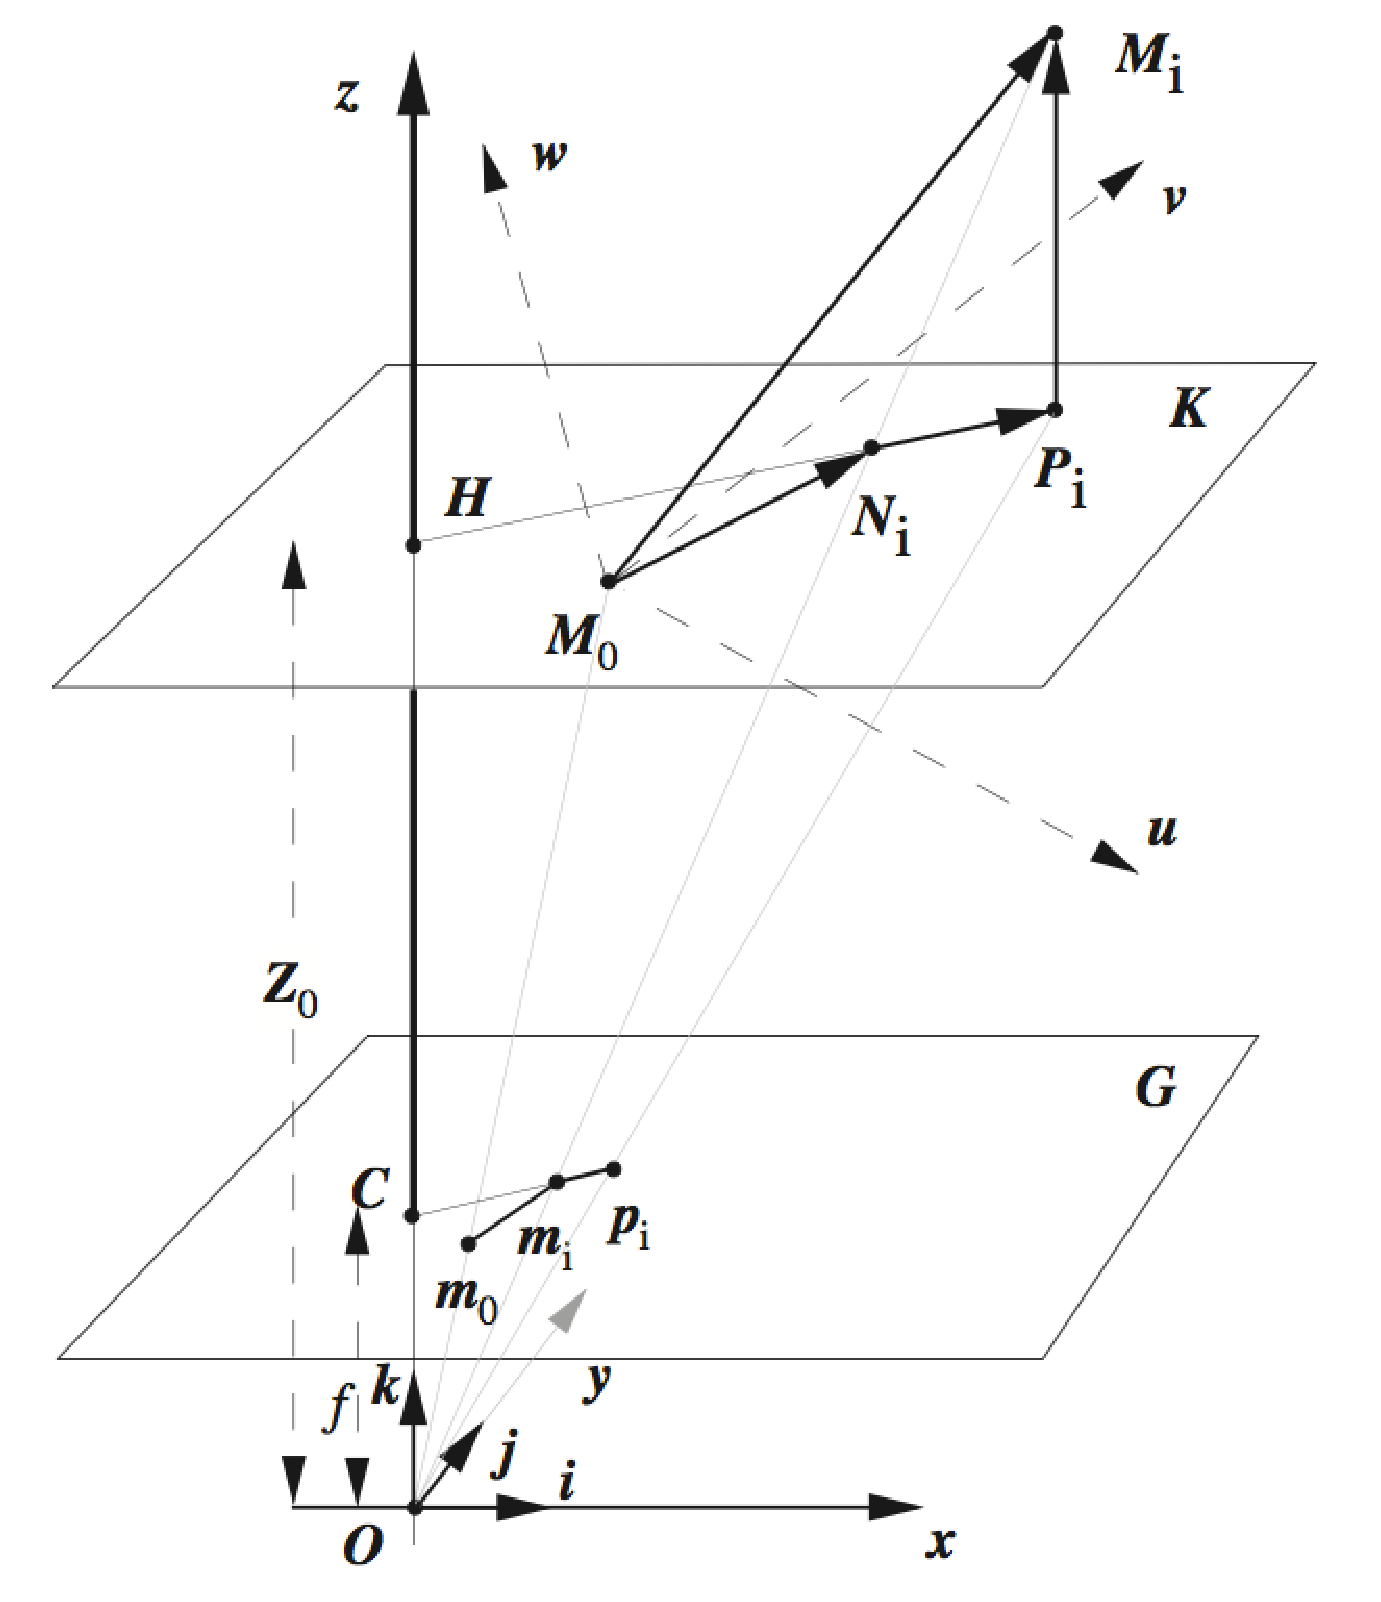
\includegraphics[scale=0.5]{figs_posit/posit_1.eps}
\caption{Proyecci�n en perspectiva ($m_i$) y SOP ($p_i$) para un punto del modelo 3D $M_i$ y un punto de referencia del modelo $M_O$. Tomado de: \cite{DeMenthon95} .}
\label{fig: posit_1}
\end{figure}

Se busca computar la matriz de rotaci�n y el vector de traslaci�n del objeto respecto a la c�mara. 
%La matriz de rotaci�n \textbf{R} del objeto, es la matriz cuyas filas son las coordenadas del los versores $i$, $j$ y $k$, expresados en el sistema de coordenadas del objeto ($u$, $v$, $w$), se puede ver como la matriz de cambio de base que pasa coordenadas en la base del objeto a coordenadas en la base de la c�mara. %
Se recuerda que matriz de rotaci�n se expresa como:
\[ R=\left( \begin{array}{ccc}
i_u & i_v & i_w \\
j_u & j_v & j_w \\
k_u & k_v & k_w \end{array} \right)\] 

Por lo tanto, para obtener la matriz de rotaci�n s�lo es necesario obtener los versores  \textbf{i}  y  \textbf{j} , el versor  \textbf{k}  se obtiene de realizar el producto vectorial  \textbf{i} $\times$  \textbf{j}. El vector de traslaci�n es el vector que va del centro del objeto $M_0$ a el centro del sistema de coordenadas de la c�mara $O$. Por lo tanto las coordenadas del vector de traslaci�n son ($X_0$,$Y_0$,$Z_0$). Si este punto $M_0$ es uno de los puntos visibles en la imagen, entonces el vector \textbf{T}  esta alineado con el vector $Om_0$ y es igual a ($Z_0$/$f$)$Om_0$. La pose queda determinada si se conocen  \textbf{i}, \textbf{j} y  \textbf{$Z_0$}.

%Como detalle a tener en cuenta, se observa que para calcular la traslaci�n es necesario conocer el punto de referencia del objeto $M_0$, esta es la principal diferencia con la versi�n moderna de POSIT en la que para calcular la traslaci�n no es necesario suponer nada acerca del punto de referencia del objeto. %

\subsection{SOP: \textit{S}caled \textit{O}rtographic \textit{P}rojection}\label{sec:classicPosit2}
La proyecci�n ortogonal escalada(SOP) es una aproximaci�n a la proyecci�n perspectiva. En esta aproximaci�n se supone que las profundidades $Z_i$ de diferentes puntos $M_i$ en el eje de coordenadas de la c�mara no difieren mucho entre s�, y por lo tanto se asume que todos los puntos $M_i$ tienen la misma profundidad que el punto $M_0$. Esta suposici�n es razonable cuando la relaci�n distancia c�mara objeto - profundidad del objeto es grande.

Para un punto $M_i$ la proyecci�n perspectiva sobre el plano imagen est� dada por:
\begin{align*}
x_i &= f X_i/Z_i,  & y_i& = fY_i/Z_i,
\end{align*}
mientras que la proyecci�n SOP est� dada por: 
\begin{align*}
x^{'}_i &= f X_i/Z_0, & y^{'}_i& = fY_i/Z_0. 
\end{align*}
De aqu� en m�s las proyecciones SOP de los puntos $M_i$ se identificar�n como $p_i$, mientras que las proyecciones perspectivas, que son los puntos que se detectan en la imagen, se identifican como $m_i$. 
Al t�rmino $s=f/Z_0$ se lo conoce como el factor de escala de la SOP. Se puede ver que para el caso particular del punto $M_0$ la proyecci�n perspectiva $m_0$ y la SOP $p_0$ coinciden. 

En la Figura \ref{fig: posit_1} se puede ver como se construye la SOP. Primero se realiza la proyecci�n ortogonal de todos los puntos $M_i$ sobre $K$, el plano paralelo al plano imagen que pasa por el punto $M_0$. Las proyecciones de los puntos $M_i$ sobre $K$ se llaman $P_i$. El segundo paso consiste en hacer la proyecci�n perspectiva de los puntos $P_i$ sobre el plano imagen $G$ para obtener finalmente los puntos $p_i$. En la figura tambi�n se puede ver que el tama\~no del vector $m_0p_i$ es $s$ veces el tama\~no de $M_0P_i$. Teniendo esto en cuenta se pueden expresar las coordenadas de $p_i$ como:
\begin{equation*}\
\begin{split}
x^{'}_i = fX_0/Z_0 + f(X_i - X_0)/Z_0 = x_0 + s(X_i - X_0)\\ 
y^{'}_i = y_0 + s(Y_i - Y_0)
\end{split}
\end{equation*}

\subsection{Ecuaciones para calcular la proyecci�n perspectiva}\label{sec:classicPosit3}

Como se mencion� anteriormente la pose queda determinada si se conocen los vectores \textbf{i},\textbf{j} y la coordenada \textbf{$Z_0$} del vector de traslaci�n. La relaci�n entre las coordenadas de los puntos $M_i$  en el sistema de coordenadas del objeto y el sistema de coordenadas de la c�mara es
\begin{equation}\label{eq_1}
 \left(\begin{array}{ccc}
 X_i \\
 Y_i \\
 Z_i \\
 \end{array}\right) 
  = \left( \begin{array}{ccc}
i_u & i_v & i_w \\
j_u & j_v & j_w \\
k_u & k_v & k_w \end{array} \right) 
 \left(\begin{array}{ccc}
 U_i \\
 V_i \\
 W_i \\
 \end{array}\right) +
  \left(\begin{array}{ccc}
 X_0 \\
 Y_0\\
 Z_0 \\
 \end{array}\right) 
\end{equation}
de esta expresi�n se tiene
\begin{equation*}
x_i = f\frac{\textbf{M}_0\textbf{M}_i\cdot\textbf{i}+X_0}{\textbf{M}_0\textbf{M}_i\cdot\textbf{k}+Z_0}
\end{equation*}
y si se saca $Z_0$ de factor com�n se tiene
\begin{equation*}
x_i = \frac{\textbf{M}_0\textbf{M}_i\cdot\frac{f}{Z_0}\textbf{i}+x_0}{\textbf{M}_0\textbf{M}_i\cdot\frac{f}{Z_0}\textbf{k}+1}.
\end{equation*}
Lo mismo se tiene para $y_i$.

Por lo tanto la condici�n necesaria para que la pose definida por \textbf{i},\textbf{j}, $x_0$, $y_0$ y $Z_0$ sea la pose exacta se puede expresar en las siguientes ecuaciones: 
\begin{equation}\label{eq_2}
\textbf{$M_0M_i$}\frac{f}{Z_0} \textbf{i}=x_i(1+\epsilon_i)-x_0
\end{equation}
\begin{equation}\label{eq_3}
\textbf{$M_0M_i$}\frac{f}{Z_0} \textbf{j}=y_i(1+\epsilon_i)-y_0
\end{equation}
donde $\epsilon_i$ se define como
\begin{equation}\label{eq_4}
\epsilon_i=\frac{1}{Z_0}\textbf{$M_0M_i$} \cdot \textbf{k}
\end{equation}
Se puede ver que los t�rminos $x_i(1+\epsilon_i)$ y $y_i(1+\epsilon_i)$ son las coordenadas $(x^{'}_i,y^{'}_i)$ de la SOP, en el caso en que la pose est� determinada. En la expresi�n de $\epsilon_i$ en la Ecuaci�n \ref{eq_4}, el producto escalar con \textbf{k} da la coordenada  \textit{z} de $M_0M_i$, $Z_i - Z_0$. Entonces se tiene que 
\begin{equation*}
(1+\epsilon_i) = \frac{Z_i - Z_0}{Z_0} + 1 = \frac{Z_i}{Z_0}
\end{equation*}
adem�s se tiene la proyecci�n perspectiva $x_i=fX_i/Z_i$, combinando las dos expresiones se tiene
\begin{equation*}
x_i(1+\epsilon_i) = f\frac{X_i}{Z_i} \frac{Z_i}{Z_0} = f\frac{X_i}{Z_0}
\end{equation*} 
que es la coordenada $x^{'}_i$ del punto $p_i$.

\subsection{Algoritmo}\label{sec:classicPosit4}
Las Ecuaciones \ref{eq_2} y \ref{eq_3} se puede reescribir como:
\begin{equation}\label{eq_8}
\textbf{$M_0M_i$} \textbf{I}=x_i(1+\epsilon_i)-x_0
\end{equation}
\begin{equation}\label{eq_9}
\textbf{$M_0M_i$} \textbf{J}=y_i(1+\epsilon_i)-y_0
\end{equation} 
en donde 
\begin{align}
\textbf{I}& = \frac{f}{Z_0}\textbf{i} = s\cdot \textbf{i},&  \textbf{J} = \frac{f}{Z_0}\textbf{j} = s\cdot\textbf{j}
\end{align}

Si se conociera el valor de $\epsilon_i$, las Ecuaciones \ref{eq_8} y \ref{eq_9} representan un sistema de ecuaciones en que las inc�gnitas son los vectores $\textbf{I}$ y $\textbf{J}$. Una vez obtenidos estos vectores se pueden obtener los versores $\textbf{i}$ y $\textbf{j}$ normalizando, y $Z_0$ se obtiene de la norma de cualquiera de los vectores  $\textbf{I}$ o $\textbf{J}$. A esta parte del del algoritmo se le llama \textit{POS} (\textit{P}ose from \textit{O}rthography and \textit{Scaling}), ya que estima la pose a partir de las proyecciones SOP de los puntos $M_i$.

Si se conocieran los valores exactos de los $\epsilon_i$ la pose obtenida de resolver el sistema de ecuaciones ser�a la pose exacta del objeto, como no se conocen los valores exactos de $\epsilon_i$ se utiliza un m�todo iterativo que converge a la soluci�n buscada. En la primera iteraci�n se le toma $\epsilon_i = 0$. La ecuaci�n para un punto cualquiera est� dada por: 
\begin{equation}\label{eq_10}
\begin{split}
M_0M_i\cdot\textbf{I} = x^{'}_i - x_0\\
M_0M_j\cdot\textbf{J} = y^{'}_i - y_0
\end{split}
\end{equation}
Si se escribe la Ecuaci�n \ref{eq_10} para los $n$ puntos del modelo, se tiene un sistema de $n$ ecuaciones con \textbf{I} y \textbf{J} como inc�gnitas
  \begin{equation}\label{eq_11}
 \begin{split}
 \textbf{A}\textbf{I} = x^{'} - x_0 \\
 \textbf{A}\textbf{J} = y^{'} - y_0
 \end{split}
 \end{equation}
\textbf{A} es una matriz $n\times3$ con las coordenadas de los puntos del modelo $M_i$ en el marco de coordenadas del objeto. Si se tienen mas de 4 puntos y no son coplanares, la matriz \textbf{A} es de rango 3, y las soluciones al sistema est�n dadas por
 \begin{equation}\label{eq_12}
 \begin{split}
 \textbf{I} = \textbf{B}\left(x^{'} - x_0\right)\\
 \textbf{J} = \textbf{B}\left(y^{'} - y_0\right)
 \end{split}
 \end{equation}
donde \textbf{B} es la pseudo inversa de la matriz \textbf{A}. Se debe notar que la matriz \textbf{B} depende �nicamente de la geometr�a del modelo que se asume conocida, por lo tanto solo es necesario calcularla una sola vez. 

Una vez obtenidos \textbf{I} y \textbf{J} se calculan \textit{s} y los versores \textbf{i}, \textbf{j} y \textbf{k}
\begin{subequations} \label{eq_13}
 \begin{align}
 s& =\left(\vert\textbf{I}\vert \vert\textbf{J}\vert\right)^{1/2} \\
 \textbf{i}& = \frac{\textbf{I}}{s} \\
 \textbf{j}& = \frac{\textbf{J}}{s} \\
 \textbf{k}& = \textbf{i} \times \textbf{j}
 \end{align}
 \end{subequations}
El vector traslaci�n del centro del objeto al centro de la c�mara es el vector $OM_0$ 
\begin{equation}\label{eq_14}
OM_0 = \frac{Z_0}{f}Om_0 = \frac{Om_0}{s}
\end{equation}
El vector $Om_0$ es conocido ya que se conocen las coordenadas de los puntos $m_i$, en particular $m_0$.

Una vez que se calcularon \textbf{i}, \textbf{j}, \textbf{k} y \textbf{T} se calculan los valores actualizados de $\epsilon_i$ seg�n la Ecuaci�n \ref{eq_4}. Si la variaci�n de los $\epsilon_i$ es mayor a un determinado umbral, se repite el procedimiento actualizando las proyecciones SOP en la Ecuaci�n \ref{eq_11}, si es menor al umbral se deja de iterar y se guarda la pose calculada.

\subsection{POSIT para puntos coplanares}\label{sec:classicPosit5}

Como se mencion� anteriormente, el algoritmo POSIT no funciona en el caso en que los puntos del modelo pertenecen a un mismo plano. Como los marcadores utilizados son planos, se busc� una versi�n de POSIT que resuelve el problema de la estimaci�n de pose para este caso. El algoritmo fue escrito por DeMenthon et al. en \cite{CoplanarPosit}.

Para entender cual es el problema de trabajar con puntos coplanares se explica la situaci�n desde un punto de vista geom�trico. Como se vio anteriormente, $$ M_0M_i\cdot\textbf{I}=x^{'}_i-x_0.$$ Esto quiere decir que si se toma que la base de \textbf{I} en \textbf{$M_0$} , la punta del vector $\textbf{I}$ se proyecta sobre el vector $M_0M_i$ en un punto ${H_x}_i$, entonces todas las posibles puntas del vector \textbf{I} se encuentran en el plano perpendicular a $M_0M_i$ que pasa por el punto ${H_x}_i$. Si se tuvieran 4 puntos no coplanares $M_0$, $M_1$, $M_2$ y $M_3$, el vector \textbf{I} quedar�a determinado. La base de \textbf{I} estar�a en $M_0$ y la punta estar�a en la intersecci�n de los planos perpendiculares a $M_0M_1$, $M_0M_2$ y $M_0M_3$ por los puntos ${H_x}_1$, ${H_x}_2$ y ${H_x}_3$ respectivamente. Para este caso el sistema definido en \ref{eq_11} es de rango 3. 
\begin{figure}[h!]
\centering
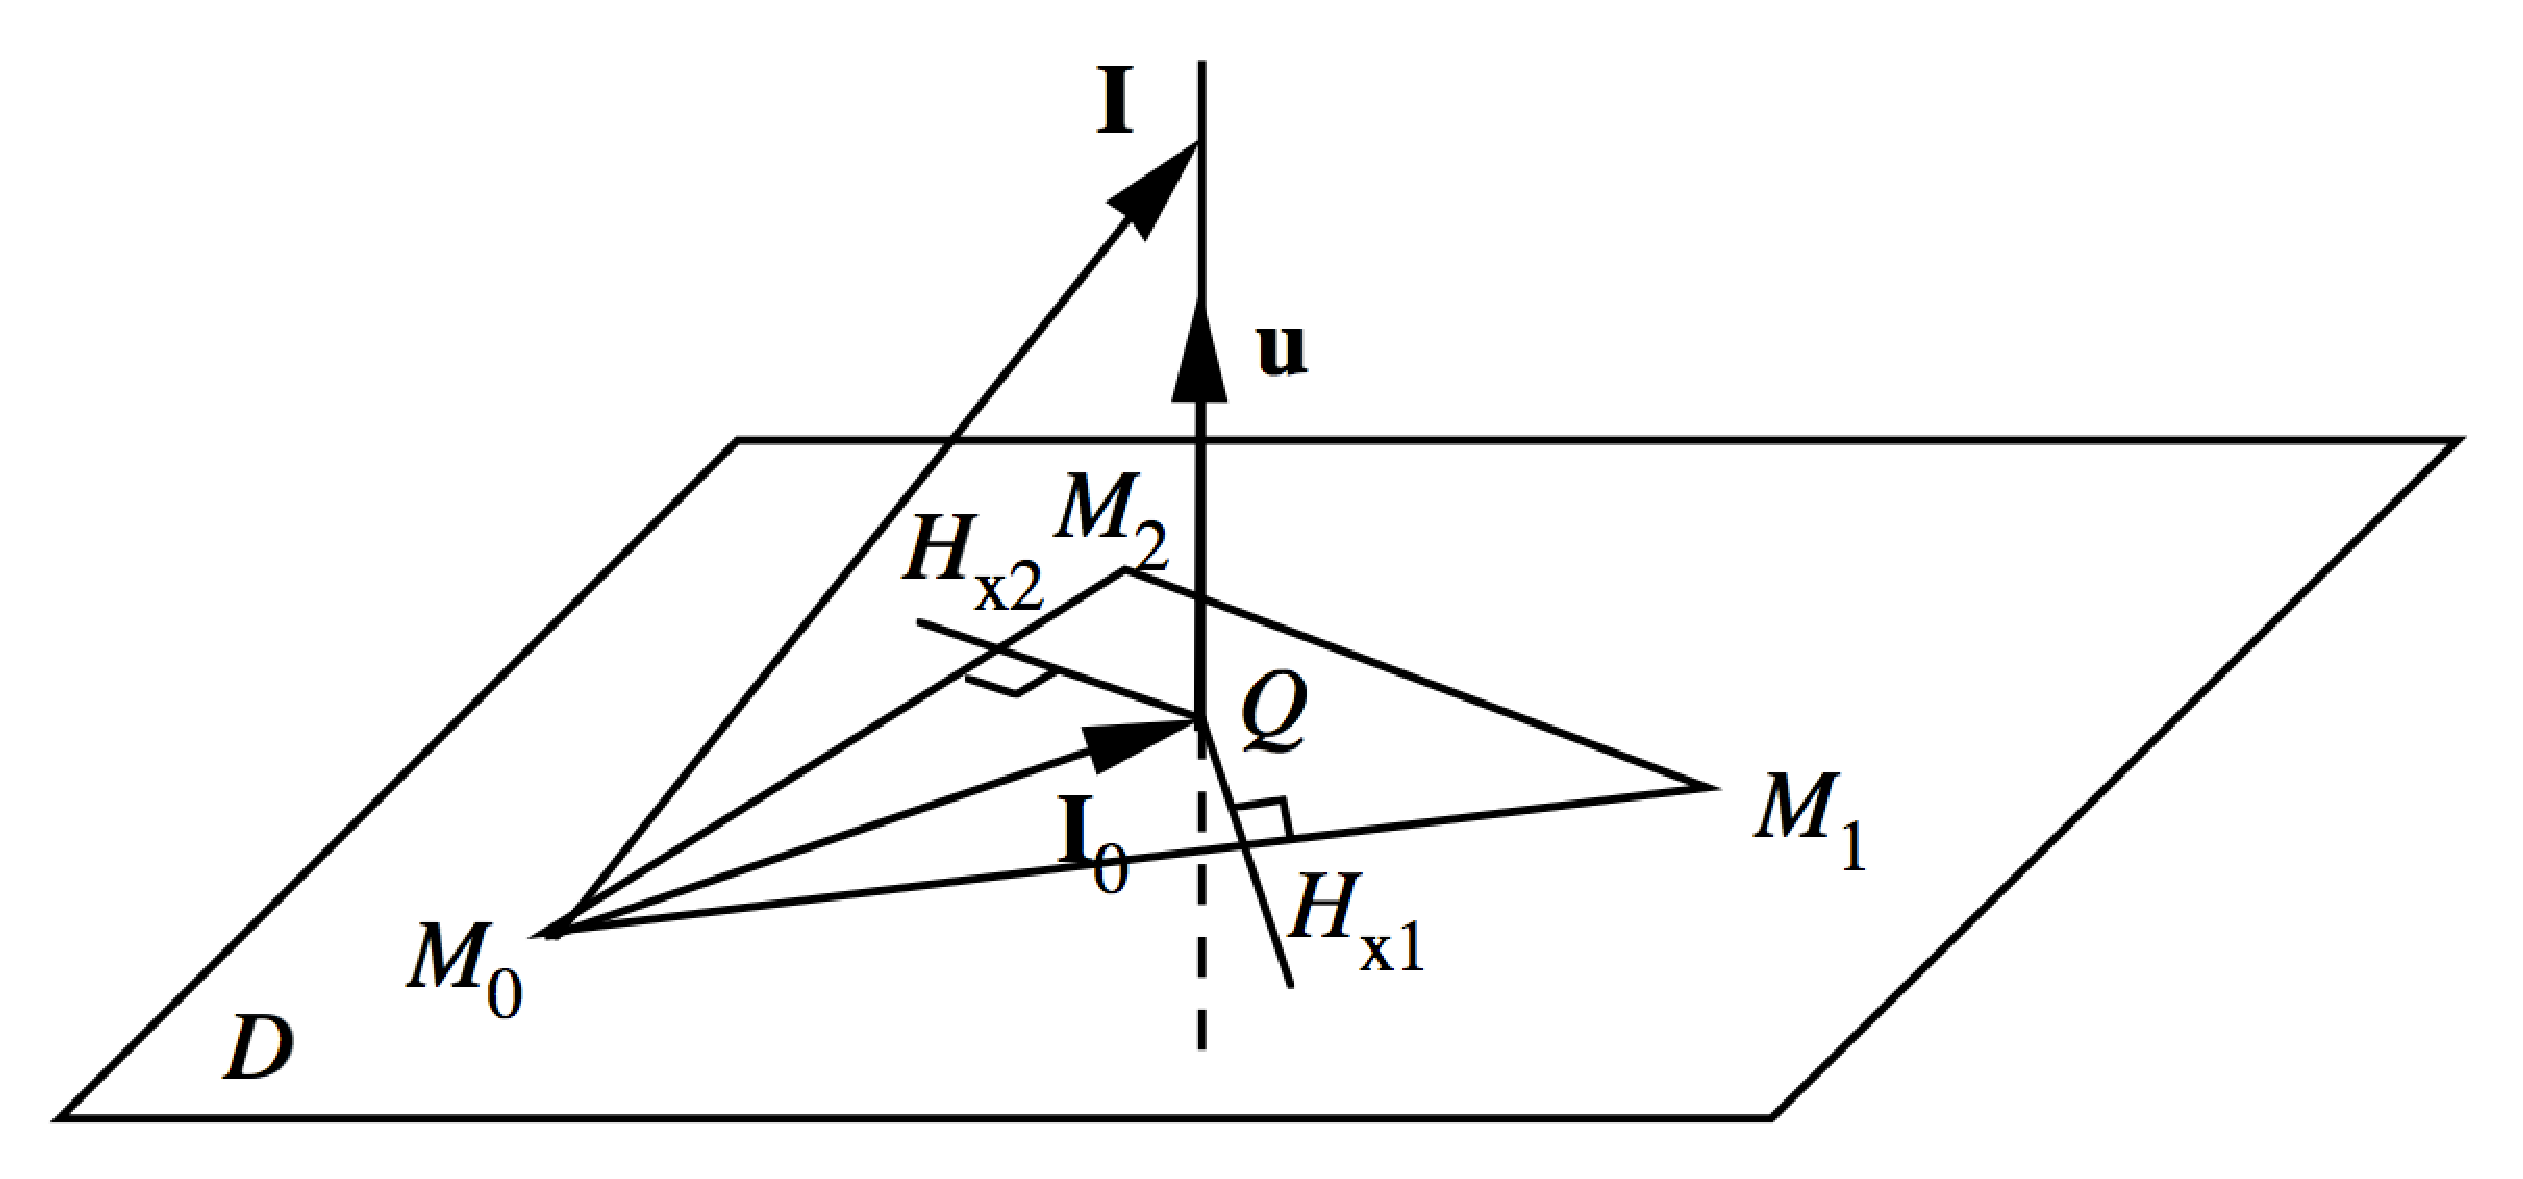
\includegraphics[scale=0.3]{figs_posit/posit_2.eps}
\caption{Configuraci�n de puntos coplanares pertenecientes al plano \textit{D}. Los planos perpendiculares que pasan por los puntos ${H_x}_1$ y ${H_x}_2$ se intersectan en un recta que pasa por el punto \textit{Q}. Se puede ver que si hubiera un $4^{to}$ punto, el plano perpendicular correspondiente har�a aparecer 2 rectas paralelas. Tomado de: \cite{CoplanarPosit} .}
\label{fig: posit_2}
\end{figure}

Si los puntos son coplanares, los vectores $M_0M_1$, $M_0M_2$ y $M_0M_3$ son todos coplanares y los planos perpendiculares que pasan por los puntos ${H_x}_1$, ${H_x}_2$ y ${H_x}_3$, se intersectan todos un una l�nea o en dos l�neas paralelas por lo tanto hay infinitas soluciones para el vector \textbf{I}. En este caso el sistema de ecuaciones en \ref{eq_11} queda de rango 2. El vector soluci�n que se obtiene al realizar la pseudo inversa de \textbf{A} es el que est� a menor distancia de los planos, en la Figura \ref{fig: posit_2} es el vector $\textbf{I}_{0}$. Esta soluci�n no es la soluci�n al problema de los vectores de rotaci�n, las soluciones se pueden expresar como
\begin{equation}\label{eq_15}
\begin{split}
\textbf{I} = \textbf{I}_{0} + \lambda \textbf{u}\\
\textbf{J} = \textbf{J}_{0}+ \mu \textbf{u}
\end{split}
\end{equation}
donde \textbf{u} es un versor perpendicular al plano de los puntos, $\textbf{J}_{0}$ se calcula de manera an�loga a $\textbf{I}_{0}$ y $\lambda$ y $\mu$ son las coordenadas de \textbf{I} y \textbf{J} seg�n el versor \textbf{u}. Para encontrar las soluciones hay que calcular el versor \textbf{u} y los valores de $\lambda$ y $\mu$.

Como el vector \textbf{u} es perpendicular al plano de los puntos caracter�sticos se cumple $M_0M_i\cdot\textbf{u}=0$, se puede hallar  entonces como la base del n�cleo de la matriz \textbf{A}. En la pr�ctica este vector se halla a partir de la descomposici�n \textit{SVD} de la matriz \textbf{A}. La descomposici�n en valores singulares de la matriz \textbf{A} queda:
\begin{equation}\label{eq_16}
A = U \Sigma V^{T}
\end{equation}
donde $U \in \Re^{n\times n}$ es ortogonal, $\Sigma \in \Re^{n \times 3}$ es diagonal, con los valores singulares en la diagonal y $V \in \Re^{3 \times 3}$ es ortogonal. Como la matriz \textbf{A} es de rango 2, los dos primeros vectores columna de la matriz V corresponden a la base de todos los puntos que pertenecen al plano del modelo, mientras que el �ltimo vector de \textbf{V} es la base del n�cleo de \textbf{A}, o sea el vector \textbf{u}. El c�lculo \textbf{u} se realiza junto al c�lculo de la matriz \textbf{B}, ya que para ambos es necesario hacer la descomposici�n \textit{SVD} de \textbf{A}. 

Para calcular los valores de $\lambda$ y $\mu$ se utilizan las condiciones de que \textbf{I} y \textbf{J} tienen que ser perpendiculares entre s� y del mismo largo. Como tienen que se perpendiculares se tiene que 
$$
\textbf{I}\cdot\textbf{J} = (\textbf{I}_{0} + \lambda \textbf{u})\cdot(\textbf{J}_{0}+ \mu \textbf{u}) = 0
$$
entonces se tiene que 
\begin{equation}\label{eq_17}
\lambda \mu = -\textbf{I}_{0} \cdot \textbf{J}_{0}
\end{equation}
Como tienen que ser del mismo largo se tiene que
\begin{equation}\label{eq_18}
(\textbf{I}_{0} + \lambda \textbf{u}) \cdot (\textbf{I}_{0} + \lambda \textbf{u}) = (\textbf{J}_{0} + \mu \textbf{u}) \cdot (\textbf{J}_{0} + \mu \textbf{u}) \Leftrightarrow \lambda^{2} - \mu^{2} = \textbf{J}_{0}^{2} - \textbf{I}_{0}^{2}
\end{equation}

Se define el n�mero complejo $C = \lambda + i\mu$, si se eleva al cuadrado queda $C^{2} = \lambda^{2} - \mu^{2} + i\lambda\mu$. Utilizando \ref{eq_17} y \ref{eq_18} se llega a que
\begin{equation}\label{eq_19}
C^{2} = \textbf{J}_{0}^{2} - \textbf{I}_{0}^{2} - 2i\textbf{I}_{0} \cdot \textbf{J}_{0}
\end{equation}
por lo que $\lambda$ y $\mu$ pueden calcularse como las partes real e imaginaria del complejo \textit{$C^{2}$}. Para hallar la ra�ces de \textit{$C^{2}$}, se expresa en forma polar:
 \begin{center}
 $C^2 = \left[R, \Theta \right],$ donde \\ 
 $ R = \left(\left(\textbf{J}_{0}^{2} - \textbf{I}_{0}^{2}\right)^2 + 4\left(\textbf{I}_0\cdot\textbf{J}_0\right)^2\right)^{1/2} $\\
 $ \Theta = \arctan\left(\dfrac{-2\textbf{I}_0\cdot\textbf{J}_0}{\textbf{J}_{0}^{2} - \textbf{I}_{0}^{2}}\right),$ si $\textbf{J}_{0}^{2} - \textbf{I}_{0}^{2}>0$, y\\
 $\Theta = \arctan\left(\dfrac{-2\textbf{I}_0\cdot\textbf{J}_0}{\textbf{J}_{0}^{2} - \textbf{I}_{0}^{2}}\right) + \pi,$ si $\textbf{J}_{0}^{2} - \textbf{I}_{0}^{2}<0$\\
 si $\textbf{J}_{0}^{2} - \textbf{I}_{0}^{2}=0$ se toma $\Theta = -sg\left(\textbf{I}_0\cdot\textbf{J}_0\right)\frac{\pi}{2},$ y $R = \vert2\textbf{I}_0\cdot\textbf{J}_0\vert$
\end{center}
Se obtienen 2 ra�ces, $C  = \left[ \rho, \theta \right]$, y $C  = \left[ \rho, \theta + \pi \right]$, donde
\begin{center}
$\rho = \sqrt{R}$, y $\theta = \frac{\Theta}{2}$
\end{center}
como se mencion� anteriormente $\lambda$ y $\mu$ son las partes real e imaginaria de \textit{C}, por lo tanto
\begin{subequations}\label{eq_20}
\begin{align}
\lambda_1& = \rho \cos \theta,  &\mu_1&  = \rho \sin \theta\label{eq_21}\\
\lambda_2& = -\rho \cos \theta, &\mu_2&  = -\rho \sin \theta\label{eq_22}
\end{align}
\end{subequations}
Esto quiere decir que se obtienen dos soluciones para \textbf{I} y \textbf{J}
\begin{subequations}\label{eq_23}
\begin{align}
\textbf{I}_1&= \textbf{I}_0 + \rho \cos \theta\textbf{u},  & \textbf{J}_1& = \textbf{J}_0 + \rho \sin \theta\textbf{u}\label{eq_23a}\\
\textbf{I}_2&= \textbf{I}_0 - \rho \cos \theta\textbf{u},   &\textbf{J}_2& = \textbf{J}_0 - \rho \sin \theta\textbf{u}\label{eq_23b}
\end{align}
\end{subequations}
Como el vector \textbf{u} es perpendicular al plano del objeto, la soluci�n encontrada en \ref{eq_23a} es sim�trica a \ref{eq_23b}.  Desde el punto de vista de la c�mara, se puede ver que las dos posibles soluciones son aquellas que tienen la misma proyecci�n SOP, este comportamiento se puede ver en la Figura \ref{fig: posit_3}. 

\begin{figure}[H]
\centering
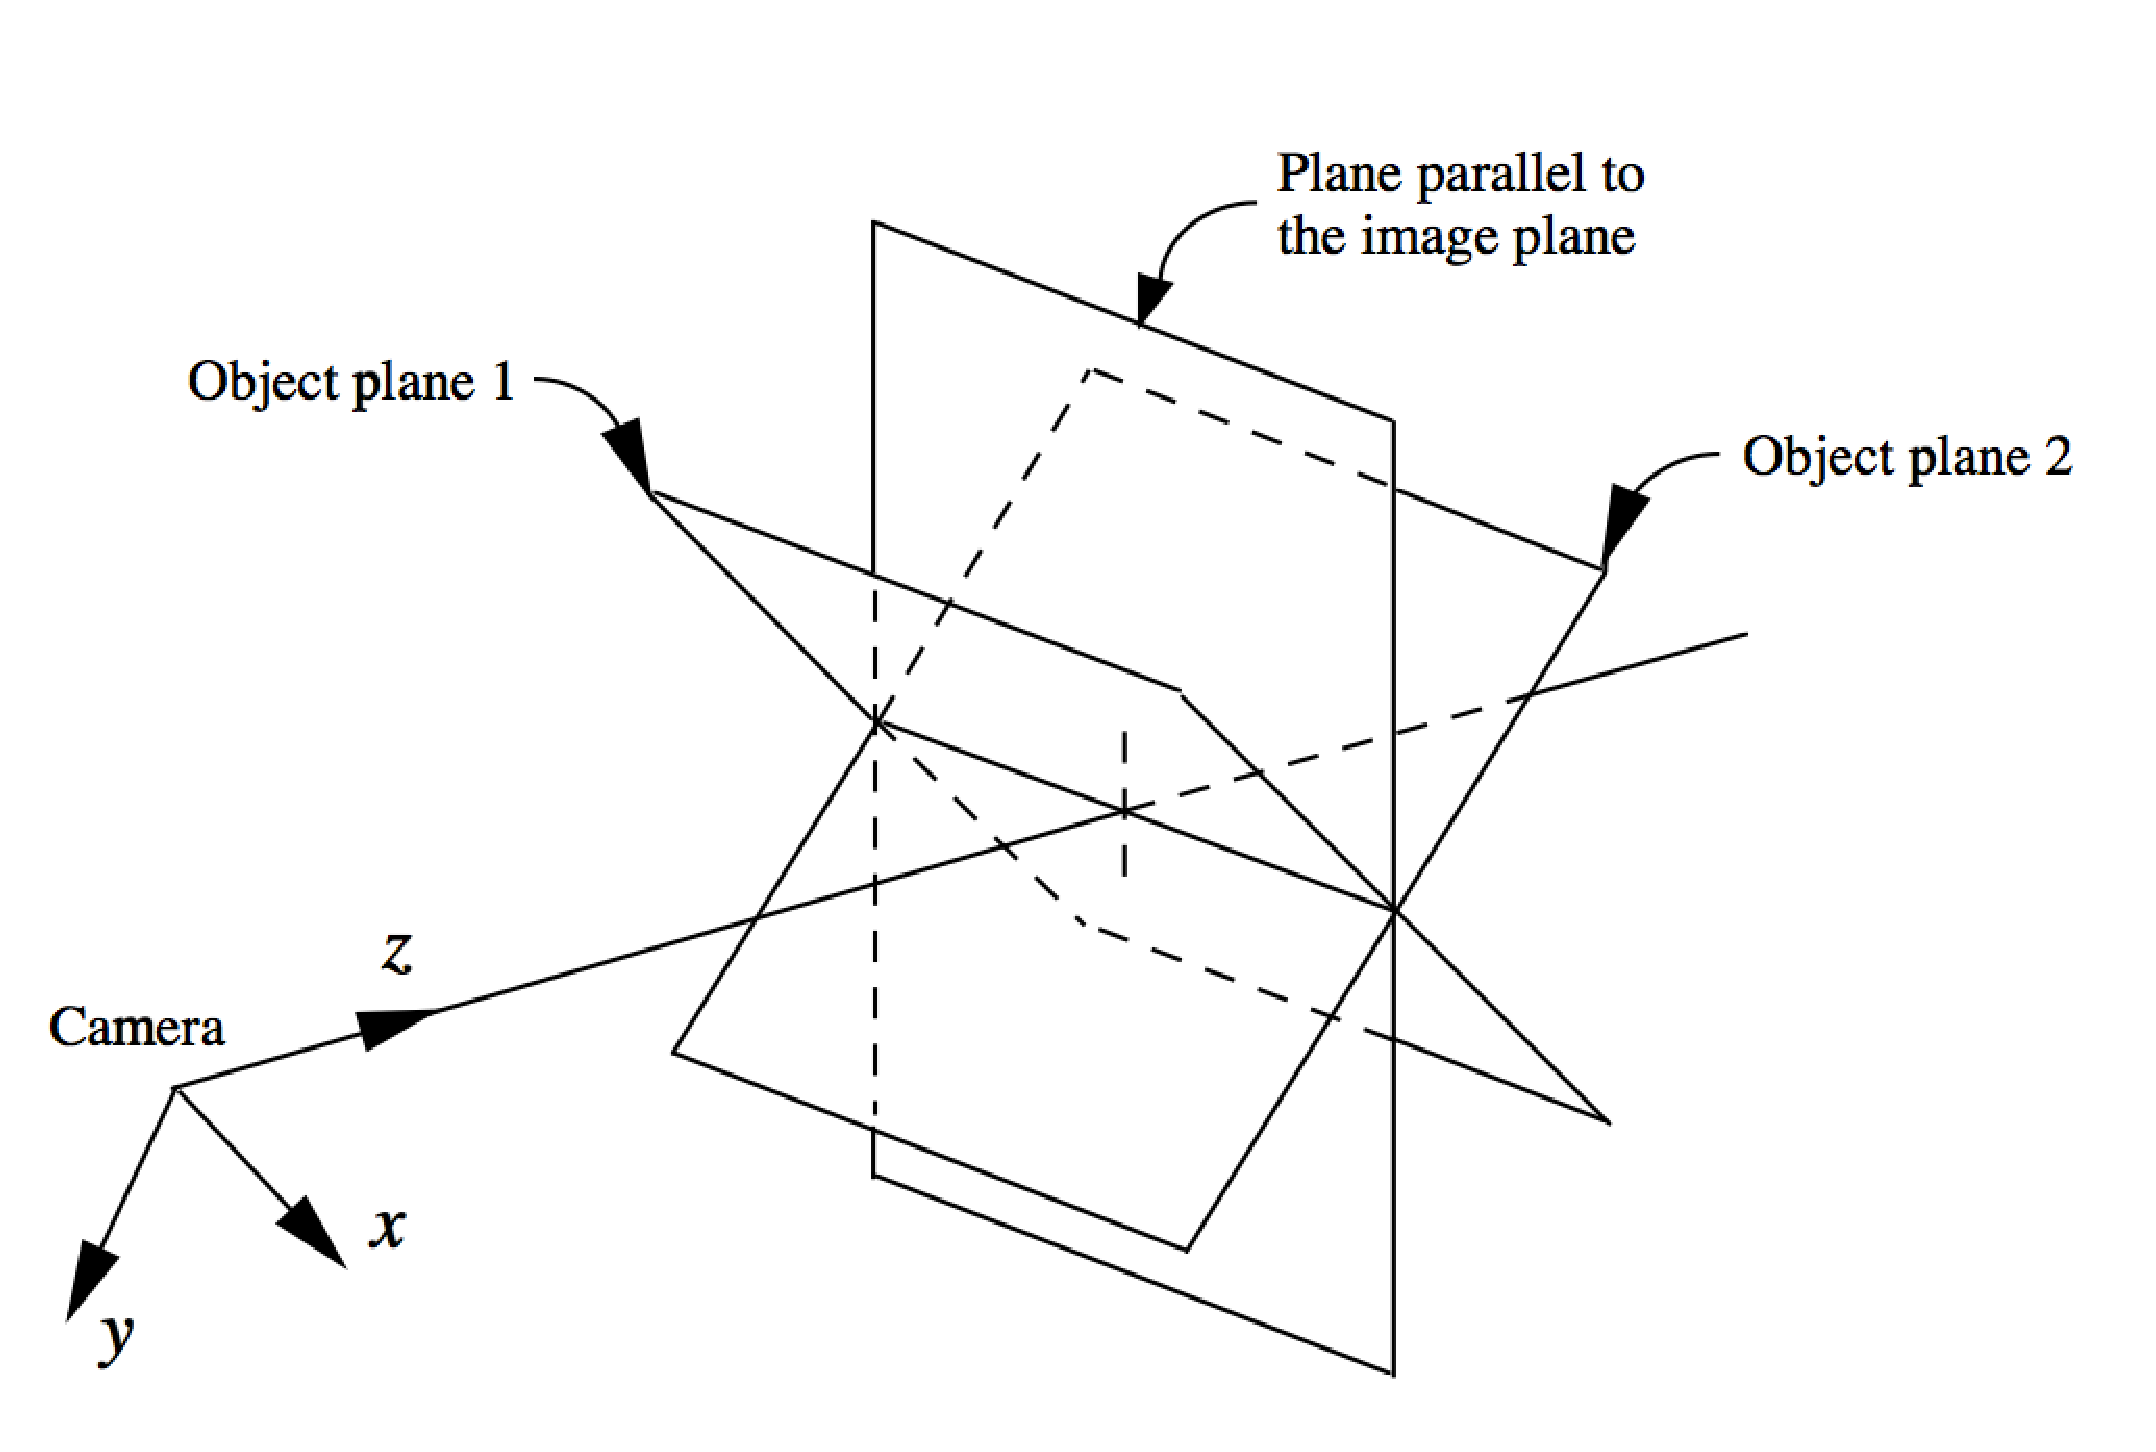
\includegraphics[scale=0.35]{figs_posit/posit_3.eps}
\caption{Dos objetos dando la misma proyecci�n SOP. Fuente: \cite{CoplanarPosit}.}
\label{fig: posit_3}
\end{figure}

Por lo tanto se toman las soluciones $(\textbf{I}_1, \textbf{J}_1)$ y $(\textbf{I}_2, \textbf{J}_2)$ y se calculan las poses. Como las dos poses son sim�tricas respecto a un plano paralelo al plano imagen, puede pasar que una pose d� una soluci�n en la que los los puntos del objeto queden ubicados detr�s de la c�mara. Por lo tanto previo a dar las dos soluciones como v�lidas hay que verificar esto.

En el caso en que las dos soluciones sean v�lidas para todas las iteraciones, el n�mero de poses posibles ser�a $2^n$ a lo largo de $n$ iteraciones. En la pr�ctica se manejan menos soluciones posibles. Se diferencian dos casos:
\begin{itemize}
\item[$\bullet$] Si se tiene que s�lo una de las dos primeras poses calculadas es v�lida, en las siguientes iteraciones se el da mismo comportamiento, por lo que hay solo un camino a seguir. Figura \ref{fig: posit_4}.

\item[$\bullet$] Si se tiene que las dos primeras poses calculadas son v�lidas, se abren dos posibles ramas. En la segunda iteraci�n cada rama da lugar a dos nuevas poses, pero en este caso se toma la pose que da menor error de reproyecci�n. Figura \ref{fig: posit_5}.

\end{itemize}

\begin{figure}[h!]
\centering
\subfigure[]{
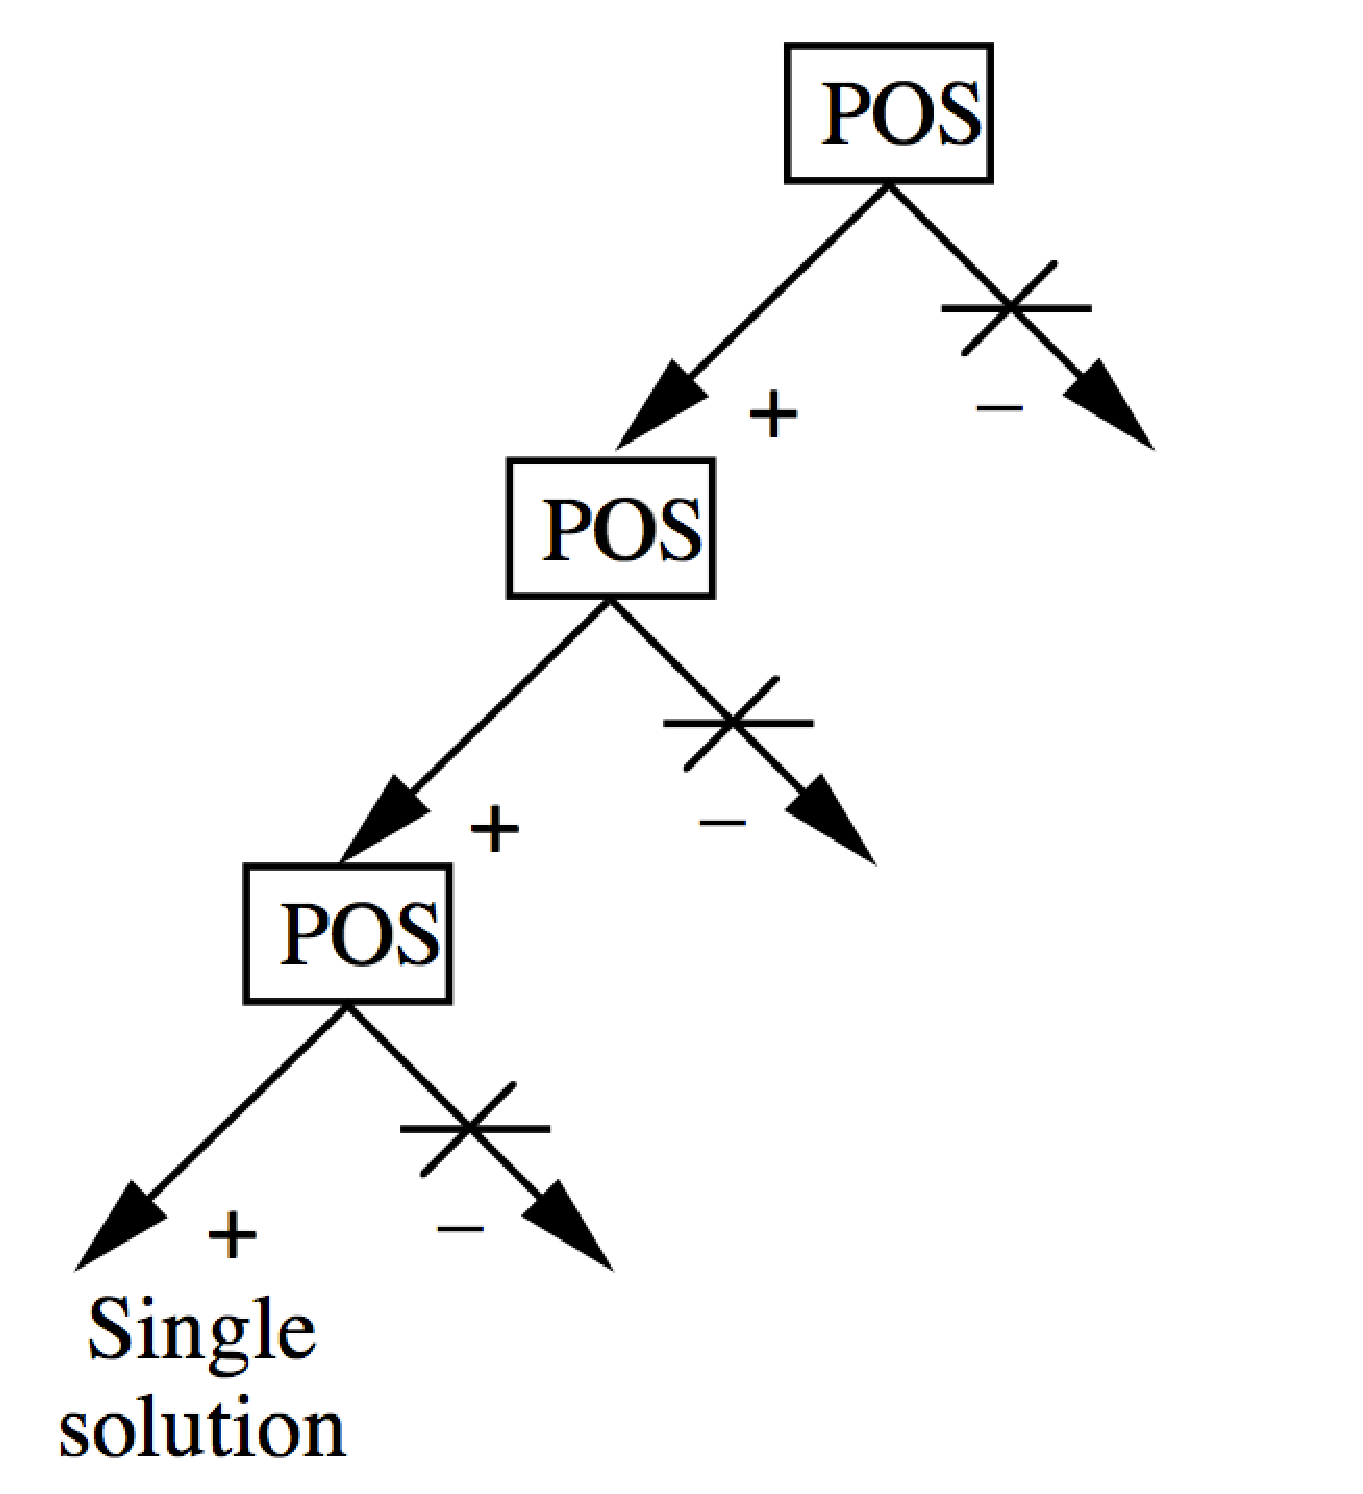
\includegraphics[scale=0.22]{figs_posit/posit_4.eps}
\label{fig: posit_4}
	}
\subfigure[]{
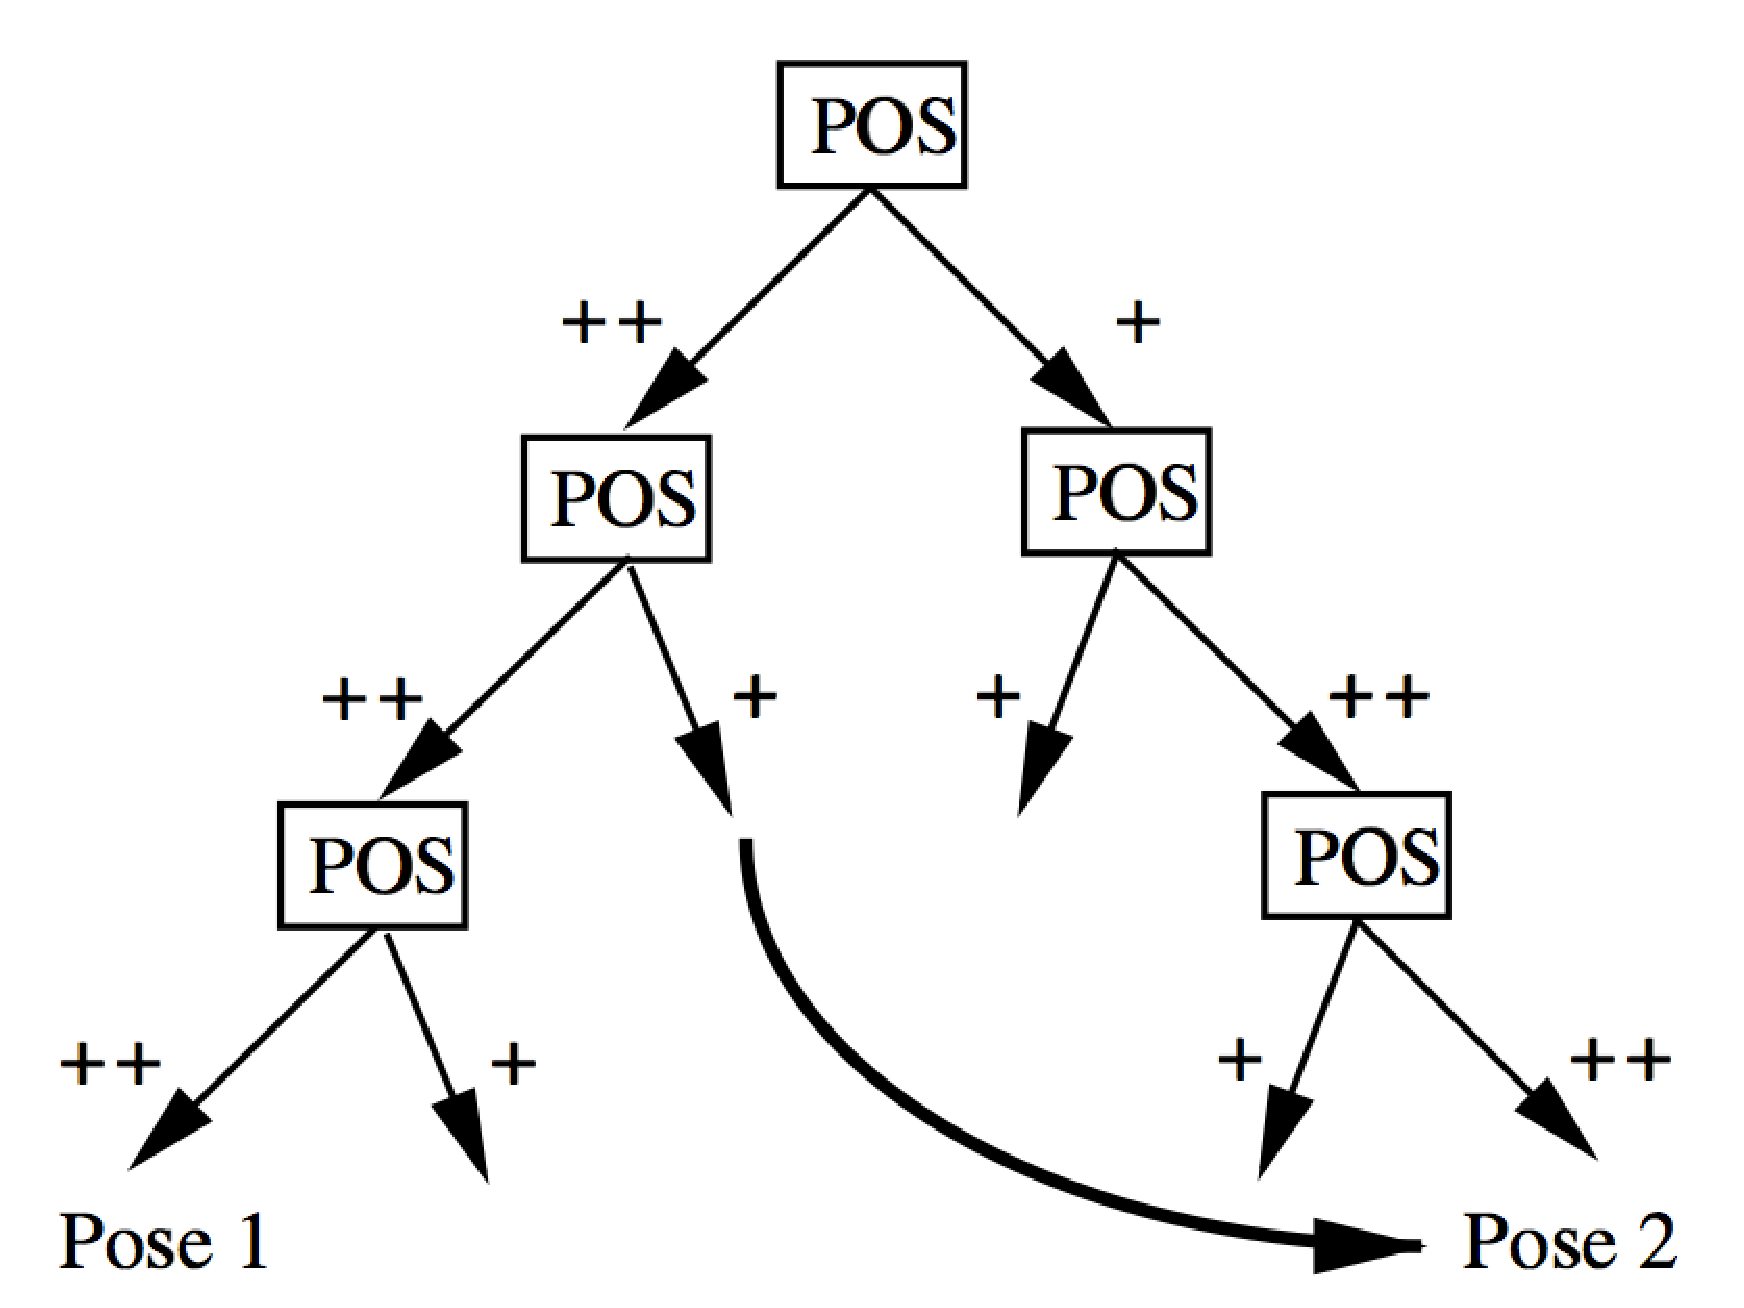
\includegraphics[scale=0.25]{figs_posit/posit_5.eps}
\label{fig: posit_5}
}
\caption{\subref{fig: posit_4}:Caso en el que solo una pose de las dos iniciales es coherente, tambi�n en las siguientes iteraciones solo una de las dos poses es posible, se tiene un �nica soluci�n. \subref{fig: posit_5}: Caso en el que en cada paso hay dos posibilidades, se opta por la mejor pose(++ mejor pose, + peor pose) en cada rama. Tomado de: \cite{CoplanarPosit}.}
\end{figure}

\begin{comment}
\begin{figure}[h!]
\centering
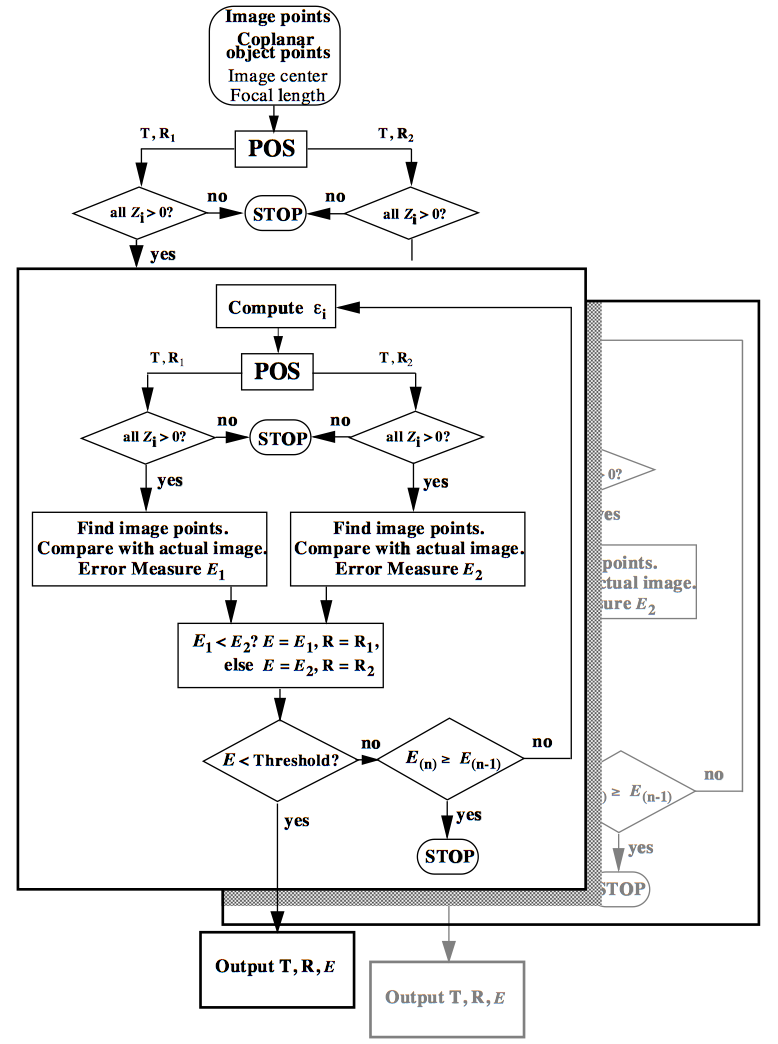
\includegraphics[scale=0.405]{figs_posit/posit_6}
\label{fig: posit_6}
\caption{Diagrama de flujo del algoritmo para puntos coplanares, \textit{E} es el error de reproyecci�n, la condici�n $Z_i>0$ verifica que los puntos reproyectados est�n por delante del plano imagen. Tomado de: \cite{CoplanarPosit}.}
\end{figure}
\end{comment}


\section{SoftPOSIT}\label{sec:SoftPosit}
Hasta aqu� se vio el algoritmo POSIT que permite obtener la pose de un modelo respecto a la c�mara para el caso en que se tienen correspondencias entre puntos del modelo y puntos caracter�sticos en la imagen. Como se vio en el cap�tulo \ref{ch:detection} obtener correspondencias entre puntos detectados en una imagen y el modelo real puede ser complicado. Por este motivo se estudi� el algoritmo SoftPOSIT desarrollado por DeMenthon et al. en \cite{Daniel03simultaneouspose}. Este algoritmo recibe como entrada los puntos del modelo 3D, una lista de puntos detectados en la imagen para los cuales no se sabe como se relacionan con los puntos del modelo y una pose inicial para realizar la b�squeda. Utiliza un m�todo llamado \textit{softassign} para resolver las correspondencias y luego que tiene las correspondencias utiliza una versi�n modificada de POSIT. 

\subsection{Modern POSIT}\label{sec:SoftPosit1}
Como se mencion� anteriormente, SoftPOSIT utiliza una versi�n modificada de POSIT llamada Modern POSIT. POSIT cl�sico requiere que se conozca cual es el punto de referencia en el modelo y en la imagen, ya que de estos datos se calcula el vector de traslaci�n. Para el caso de SoftPOSIT no es posible saber de antemano cual es el punto de referencia del modelo ya que no se tienen las correspondencias. Modern POSIT calcula la pose, sabiendo las correspondencias, pero sin utilizar ning�n punto en particular como referencia. 

El punto $M_0$ origen del sistema de coordenadas del objeto no es conocido, por lo tanto tampoco se conoce su correspondiente $m_0$ en el plano imagen. En la Ecuaci�n \ref{eq_10} que se present� en la secci�n \ref{sec:classicPosit4} se conoc�an las coordenadas del punto $m_0$, por lo que las inc�gnitas de esta ecuaci�n eran solamente los vectores \textbf{i}, \textbf{j}. 
\begin{equation*}
\begin{split}
M_0M_i\cdot\textbf{I} = x^{'}_i - x_0\\
M_0M_j\cdot\textbf{J} = y^{'}_i - y_0
\end{split}
\end{equation*}
En este caso no se conocen las coordenadas de $m_0$, por lo que tambi�n hace falta calcularlas para obtener el vector de traslaci�n. Sabiendo que \begin{equation*}
\begin{split}
X_0 = x_0/s \\
Y_0 = y_0/s
\end{split}
\end{equation*}
se puede reescribir la Ecuaci�n \ref{eq_10} como
\begin{equation}\label{eq_24}
\begin{split}
x^{'}_i = M_0M_i\cdot s\textbf{i} + sX_0\\
y^{'}_i = M_0M_j\cdot s\textbf{j} + sY_0
\end{split}
\end{equation}
El sistema a resolver queda
\begin{equation}\label{eq_25}
 \textbf{A}\cdot \left[ \begin{array}{cc}
\textbf{I} & \textbf{J} \\
sX_0 & sY_0 \end{array} \right] = \left[ \begin{array}{cc}
x^{'} & y^{'} \end{array} \right] 
\end{equation}
donde la matriz  \textbf{A} son los puntos del modelo 3D en coordenadas homog�neas. Este sistema se puede resolver utilizando m�nimos cuadrados, como se vio en la secci�n \ref{sec:classicPosit4}.%%Se calcula la pseudo inversa de la matriz \textbf{A} y luego se obtienen \textbf{i}, \textbf{j} y \textbf{k} como se vi� en \ref{eq_13}. Finalmente el vector de traslaci�n se obtiene como.
%\begin{align}\label{eq_26}
%X_0 &= \frac{(sX_0)}{s}& Y_0 &= \frac{(sY_0)}{s}& Z_0 &= \frac{f}{s} 
%\end{align} 

Sin embargo se propone un m�todo que busca minimizar la distancia al cuadrado entre las proyecciones SOP de los puntos $M_i$ y las proyecciones SOP calculadas en cada iteraci�n. En la Figura \ref{fig: posit_7} se puede ver geom�tricamente cual es la distancia que se busca minimizar.
\begin{figure}[h!]
\centering
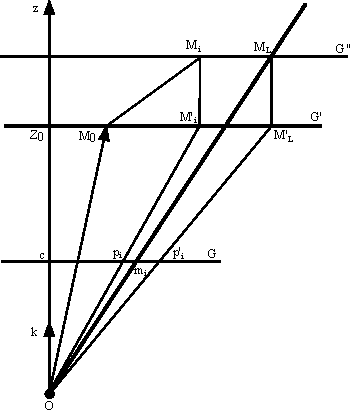
\includegraphics[scale=1.5]{figs_posit/posit_7}
\label{fig: posit_7}
\caption{Interpretaci�n geom�trica de POSIT. El punto $p_i$ es la proyecci�n SOP de $M_i$ que es el t�rmino de la derecha de la Ecuaci�n \ref{eq_24}. El punto $p^{'}_i$ es la proyecci�n SOP de $M_L$, ubicado en la l�nea de vista de $m_i$, corresponde al t�rmino de la izquierda de la Ecuaci�n \ref{eq_24}. Para que la ecuaci�n se satisfaga se tiene que cumplir que $p_i$ y $p^{'}_i$ sean iguales. Fuente: \cite{Daniel03simultaneouspose}.}
\end{figure}

En el t�rmino de la derecha de la Ecuaci�n \ref{eq_24} se tiene la proyecci�n SOP de $M_i$, $p_i$. Las coordenadas de este punto son
$$ p_i = s(M_0M_i\cdot \textbf{i} + X_0 , M_0M_i\cdot \textbf{j} + Y_0).$$
Por otro lado, en el t�rmino de la izquierda de \ref{eq_24} se tienen las coordenadas del punto $p^{'}_i$ 
$$ p^{'}_i = (1 + \epsilon_i)(x_i, y_i).$$
que es la proyecci�n SOP de la intersecci�n de la l�nea de vista del punto $m_i$ con el plano $G''$, esto esta demostrado en \cite{David02softposit}. La pose encontrada es correcta cuando ambos lados de la Ecuaci�n \ref{eq_24} son iguales. Por lo tanto la ecuaci�n que se busca minimizar es la siguiente:
\begin{equation}\label{eq_27}
E = \sum _i \left( \left( \textbf{Q}_1 \cdot M_0M_i - (1+ \epsilon_i)x_i \right) ^2 + \left( \textbf{Q}_2 \cdot M_0M_i - (1+ \epsilon_i)y_i \right) ^2 \right)
\end{equation}
donde 
\begin{equation}\label{eq_28}
\begin{split}
\textbf{Q}_1 = s(i,X_0)\\
\textbf{Q}_2 = s(j,Y_0)
\end{split}
\end{equation}
y $M_0M_i$ se toma en coordenadas homog�neas. 

Los vectores $\textbf{Q}_1$ y $\textbf{Q}_2$ son aquellos que minimizan el valor $E$, por lo tanto se despejan de derivar la expresi�n de $E$ e igualarla a cero. 
\begin{comment}
\begin{equation*}
\begin{split}
\frac{\partial E}{\partial \textbf{Q}_1} = \dfrac{\partial}{\partial \textbf{Q}_1}  \left[\sum _i \left( \left( \textbf{Q}_1 \cdot M_0M_i - (1+ \epsilon_i)x_i \right) ^2 + \left( \textbf{Q}_2 \cdot M_0M_i - (1+ \epsilon_i)y_i \right) ^2 \right)\right]\\ =\sum_i  2\left( \textbf{Q}_1 \cdot M_0M_i - (1+ \epsilon_i)x_i \right) \dfrac{\partial }{\partial \textbf{Q}_1}\left(\textbf{Q}_1 \cdot M_0M_i\right) = \sum_i  2\left( \textbf{Q}_1 \cdot M_0M_i - (1+ \epsilon_i)x_i \right) M_0M_i^T = 0 
\end{split}
\end{equation*}
desarrollando el t�rmino a la izquierda y despejando se tiene que:
\begin{equation*}
\sum_i \left(\textbf{Q}_1 \cdot M_0M_i M_0M_i^T\right) = \sum_i \left( (1+ \epsilon_i)x_i M_0M_i^T\right)
\end{equation*}
si se pasa $\textbf{Q}_1$  para afuera de la sumatoria y se despeja queda:
\begin{equation}\label{eq_29}
\textbf{Q}_1 = \left(\sum_i M_0M_i M_0M_i^T\right)^{-1}\left(\sum_i \left(1+ \epsilon_i\right)x_i M_0M_i^T\right)
\end{equation}
\end{comment}
La expresi�n para calcular  $\textbf{Q}_1$ y $\textbf{Q}_2$ queda:
\begin{equation}\label{eq_30}
\textbf{Q}_1 = \left(\sum_i M_0M_i^T M_0M_i\right)^{-1}\left(\sum_i \left(1+ \epsilon_i\right)x_i M_0M_i\right)
\end{equation}
\begin{equation}\label{eq_31}
\textbf{Q}_2 = \left(\sum_i M_0M_i^T M_0M_i\right)^{-1}\left(\sum_i \left(1+ \epsilon_i\right)y_i M_0M_i\right)
\end{equation}
La matriz $L = \left(\sum_i M_0M_i^T M_0M_i\right)$ es una matriz $4 \times 4$ y como s�lo depende de los puntos del modelo puede ser calculada previamente.

Para calcular la pose se procede como sigue:
\begin{itemize}
\item[(1)] Se calculan los vectores $\textbf{Q}_1$ y $\textbf{Q}_2$ asumiendo que se conocen los valores de $\epsilon_i$, para el paso inicial se supone que $\epsilon_i = 0$.

\item[(2)] Con los vectores $\textbf{Q}_1$ y $\textbf{Q}_2$ calculados se calculan los $\epsilon_i$ corregidos. 
\end{itemize}
Cuando $E$ es menor a determinado umbral el algoritmo se detiene y se obtiene la pose. 

\subsection{C�lculo de pose sin correspondencias}\label{sec:SoftPosit2}
Se tienen \textit{N} puntos detectados en la imagen y \textit{M} puntos en el modelo. Cuando no se conocen las correspondencias cada punto detectado $m_j$ es candidato a corresponderse con cualquier punto del modelo $M_i$. La distancia que se busca minimizar es 
\begin{equation*}
d^2_{ji} = \left(\textbf{Q}_1 \cdot M_iM_0 - \left(1+\epsilon_i\right) x_j\right)^2 + \left(\textbf{Q}_2 \cdot M_iM_0 - \left(1+\epsilon_i\right) y_j\right)^2
\end{equation*}
Se puede ver que para cada punto de modelo hay \textit{N} candidatos, la distancia $d^2_{ji}$ da una idea de que tan cerca esta de ser el correspondiente. 
Para resolver el problema de estimar la pose y las correspondencias simult�neamente se busca minimizar la siguiente funci�n:
\begin{multline}\label{eq_32}
E = \sum_{j=1}^N \sum_{i=1}^M a_{ji}(d^2_{ji} - \alpha)\\
  = \sum_{j=1}^N \sum_{i=1}^M a_{ji}\left( \left( \textbf{Q}_1 \cdot M_0M_i - (1+ \epsilon_i)x_j \right) ^2 + \left( \textbf{Q}_2 \cdot M_0M_i - (1+ \epsilon_i)y_j \right) ^2 - \alpha\right)
\end{multline}
donde $a_{ji}$ son pesos para cada una de las distancias $d^2_{ji}$. Los pesos $a_{ji}$ forman lo que se llama matriz de asignaci�n, en esta matriz se puede ver el grado de correspondencia de cualquier punto detectado con cualquier punto del modelo. El valor $\alpha$ es la tolerancia que se le da a la medida de distancia.

Las expresiones para los vectores $\textbf{Q}_1$ y $\textbf{Q}_2$ se modifican
\begin{equation}\label{eq_33}
\textbf{Q}_1 = \left(\sum_{i=1}^M a^{'}_i M_0M_i^T M_0M_i\right)^{-1}\left(\sum_{j=1}^N \sum_{i=1}^M a_{ji} \left(1+ \epsilon_i\right)x_j M_0M_i\right)
\end{equation}
\begin{equation}\label{eq_34}
\textbf{Q}_2 = \left(\sum_{i=1}^M a^{'}_i M_0M_i^T M_0M_i\right)^{-1}\left(\sum_{j=1}^N \sum_{i=1}^M a_{ji} \left(1+ \epsilon_i\right)y_j M_0M_i\right)
\end{equation}
donde $a^{'}_i = \sum_{j=1}^N a_{ji}$. El t�rmino $L = \sum_{i=1}^M a^{'}_i M_0M_i^T M_0M_i $ es una matriz $4\times 4$, para este caso \textit{L} no se puede calcular previamente porque la matriz de asignaci�n cambia en cada iteraci�n.

Para minimizar \textit{E} se procede como sigue:
\begin{itemize}
\item[(1)] Se calculan las variables de la matriz de asignaci�n asumiendo todo lo dem�s conocido.

\item[(2)] Se calculan los vectores $\textbf{Q}_1$ y $\textbf{Q}_2$ asumiendo que se conocen los valores de $\epsilon_i$. Para el paso inicial se supone que $\epsilon_i = 0$.

\item[(3)] Con los vectores $\textbf{Q}_1$ y $\textbf{Q}_2$ calculados se calculan los $\epsilon_i$ corregidos. 
\end{itemize}
Esto se repite hasta que la pose converge. \\

Este algoritmo realiza la b�squeda a partir de una pose inicial. La funci�n de costo que se busca minimizar, presentada en la Ecuaci�n \ref{eq_32}, presenta m�nimos locales. La t�cnica de \textit{softassign} suaviza esta funci�n de costo por lo que muchos m�nimos locales se evitan. Sin embargo no siempre es posible suavizar la funci�n de costo hasta tener un solo el m�nimo global, y mucho suavizado hacer que se pierda el m�nimo global. Es importante entonces contar con una buena pose inicial para que el resultado sea el correcto. Otro enfoque que se presenta en \cite{Daniel03simultaneouspose} es el de correr  el algoritmo varias veces con poses iniciales aleatorias y llegar as� al m�nimo global. 

\subsection{Matriz de asignaci�n}\label{sec:SoftPosit3}
Se busca tener una matriz \textit{a} que indique las correspondencias entre los \textit{N} puntos detectados y los \textit{M} puntos en del modelo y adem�s minimice \textit{E}. 
La matriz de asignaci�n tiene las siguientes caracter�sticas:
\begin{itemize}
\item[$\bullet$] Tiene \textit{N+1} filas y \textit{M+1} columnas.
\item[$\bullet$] $a_{ji}\in\left[0,1\right]$. Si $a_{ji} = 1$ quiere decir que el punto detectado $m_j$ se corresponde con el punto del modelo $M_i$.
\item[$\bullet$] La fila \textit{N+1} y la columna \textit{M+1} se utilizan para ver si hay alguna correspondencia en esa fila o columna. Por ejemplo si el elemento \textit{j} de la columna \textit{M+1} es 1, significa que el punto detectado $m_j$ no se corresponde con ning�n punto del modelo. 
\item[$\bullet$] La suma de los elementos a los largo de cualquier fila o columna es siempre 1. 
\end{itemize}
Para obtener una matriz \textit{a} que cumpla con las caracter�sticas mencionadas se utiliza una t�cnica llamada \textit{softassign}. Se comienza con una matriz $a^0$ en la que los elementos est�n dados por
\begin{equation*}
a^0_{ji} = e^{-\beta\left(d^2_{ji} - \alpha\right)}
\end{equation*}
en donde $\beta$ es una constante muy peque\~na y la fila $N+1$ y la columna $M+1$ son inicializadas con constantes peque\~nas. Luego se itera utilizando los siguientes pasos hasta obtener la matriz \textit{a}.
\begin{itemize}
\item[(1)] Se normaliza cada fila y columna por la suma de los elementos de esa fila o columna respectivamente hasta que $\Vert a^i - a^{i-1}\Vert$ sea peque\~no. La matriz resultante cumple que todas la filas y columnas suman 1.
\item[(2)] Se incrementa el valor de $\beta$ a medida que se itera. A medida que se agranda $\beta$ cada fila y columna de $a^0$ es renormalizada, los t�rminos $a^0_{ji}$ correspondientes a las $d^2_{ji}$ convergen a 1, mientras que los dem�s convergen a 0.
\end{itemize}
Al final del algoritmo se observa que la matriz \textit{a} est� muy cerca de ser una matriz binaria indicando las correspondencias.  

\subsection{Implementaci�n}
Durante la investigaci�n de este algoritmo se desarrollaron versiones de POSIT moderno y SoftPOSIT en C. Ambas implementaciones son autocontenidas, no se necesita ninguna librer�a adicional para poderlas usar. Adem�s todas las funciones est�n incluidas en un solo archivo. Esto es de gran valor ya que no se encontr� en la web una versi�n de estos algoritmos que fuera del tipo \textit{plug and play} como lo son estas. 
 
\section{POSIT moderno para puntos coplanares}
La implementaci�n que se us� en la aplicaci�n es el POSIT moderno adaptado para trabajar con puntos coplanares. Inicialmente se quiso desarrollar una versi�n de SoftPOSIT que trabajara con puntos coplanares, para ello previamente se desarroll� POSIT moderno coplanar a modo de prueba. 

Como se vio en la secci�n \ref{sec:classicPosit5} cuando los puntos son coplanares, al resolver el sistema \ref{eq_11} se obtienen las proyecciones de los vectores \textbf{i} y \textbf{j} sobre el plano del objeto. Se utiliz� el enfoque de POSIT moderno para hallar las proyecciones de \textbf{i} y \textbf{j} sobre el plano del modelo, as� como los componentes en \textit{x} e \textit{y} del vector de traslaci�n. Luego aplicando lo visto en POSIT para puntos coplanares se termino de calcular la pose. 

Se definen los puntos $M_0M_i^*$ como los puntos $M_0M_i$ sin la coordenada \textit{z}, ya que la coordenada \textit{z} es funci�n de \textit{x} e \textit{y}. A su vez se definen los vectores $\textbf{Q}_1^*$ y $\textbf{Q}_2^*$ como los vectores $\textbf{Q}_1$ y $\textbf{Q}_2$ sin la componente seg�n el eje \textit{w} en el sistema de coordenadas del modelo. Teniendo esto en cuenta se tiene 
\begin{equation*}
E^* = \sum _i \left( \left( \textbf{Q}_1^* \cdot M_0M_i^* - (1+ \epsilon_i)x_i \right) ^2 + \left( \textbf{Q}_2^* \cdot M_0M_i^* - (1+ \epsilon_i)y_i \right) ^2 \right)
\end{equation*}
Los vectores $\textbf{Q}_1^*$ y $\textbf{Q}_2^*$ se calculan de
\begin{equation*}
\textbf{Q}_1^* = \left(\sum_{i=1}^M m^{'}_i M_0M_i^{*T} M_0M_i^*\right)^{-1}\left(\sum_{j=1}^N \sum_{i=1}^M m_{ji} \left(1+ \epsilon_i\right)x_j M_0M_i^* \right)
\end{equation*}
\begin{equation*}
\textbf{Q}_2^* = \left(\sum_{i=1}^M m^{'}_i M_0M_i^{*T} M_0M_i^*\right)^{-1}\left(\sum_{j=1}^N \sum_{i=1}^M m_{ji} \left(1+ \epsilon_i\right)y_j M_0M_i^* \right)
\end{equation*}
En este caso el t�rmino $L = \sum_{i=1}^M m^{'}_i M_0M_i^{*T} M_0M_i^* $ es una matriz $3\times 3$.
Una vez que se tienen los vectores $\textbf{Q}_1^*$ y $\textbf{Q}_2^*$ se procede como se vio en la secci�n \ref{sec:classicPosit5}

Esta implementaci�n de POSIT para puntos coplanares dio resultados levemente mejores que la versi�n obtenida de \cite{DeMenthonCoplanarCode}. Es una variante de POSIT coplanar que no se encuentra en la bibliograf�a, permite obtener la pose minimizando una funci�n de costo a diferencia de POSIT cl�sico que usa m�nimos cuadrados. 

Adem�s desde el punto de vista de programaci�n se mejor� en la interfaz respecto a la versi�n cl�sica. En la versi�n cl�sica se tiene varios archivos con las diferentes funciones que se necesitan, puede llegar a ser dif�cil entender por completo la arquitectura del algoritmo y el c�digo esta comentado en franc�s. En cambio en la versi�n implementada para este proyecto se busco tener un solo archivo con todas las funciones y mejorar la arquitectura respecto a la versi�n anterior. 

\section{Resultados}\label{sec: resultadosPosit}
Se realiz� una comparaci�n entre la implementaci�n en C de POSIT cl�sico para puntos coplanares, obtenida de \cite{DeMenthonCoplanarCode} , y una versi�n desarrollada para esta aplicaci�n de POSIT moderno para puntos coplanares. 

En una primera instancia se utilizaron im�genes sint�ticas para las cuales se cuenta con la informaci�n de la pose. Con estas poses se proyectaron los puntos del modelo sobre las im�genes y se aplic� el algoritmo para los puntos del modelo y sus proyecciones. Se busc� evaluar los algoritmos de manera aislada y no como parte del proceso completo. Este an�lisis ayud� a elegir el algoritmo a utilizar. 

Luego se utilizaron im�genes reales capturadas con el \textit{iPad 2} e im�genes sint�ticas y se les aplic� todo el proceso. Para estas im�genes se calcul� el error de reproyecci�n entre los puntos a la entrada de POSIT y los puntos reproyectados por la pose obtenida. 

\subsection{Error en pose}
En esta secci�n se analiza el error de estimaci�n obtenido de las diferentes implementaciones. Se trabaj� �nicamente con im�genes sint�ticas, para cada pose estimada se la compara con la pose utilizada para generar la imagen. Se definen dos tipos de errores: el \textit{error de orientaci�n} que es la diferencia entre los �ngulos de la pose real y la pose estimada, y el \textit{error de posici�n} es la diferencia entre la posici�n del centro del objeto calculado y el real. Se utiliz� un conjunto de 360 im�genes. 180 im�genes simulan el marcador a 1m de distancia y se utilizan rotaciones entre $[-30^\circ,30^\circ]$ en torno a todos los ejes. Para las otras 180 im�genes se toman las mismas rotaciones pero la distancia al marcador es de 1.5m. 

Se estudia cu�l es el rango de funcionamiento de los algoritmos, es decir para qu� orientaciones y posiciones el algoritmo estima la pose correctamente.

\subsubsection{Error de orientaci�n}
En la Figura \ref{fig:posit_8}se muestran los resultados obtenidos para el error en orientaci�n.  

\begin{figure}[H]
\centering
        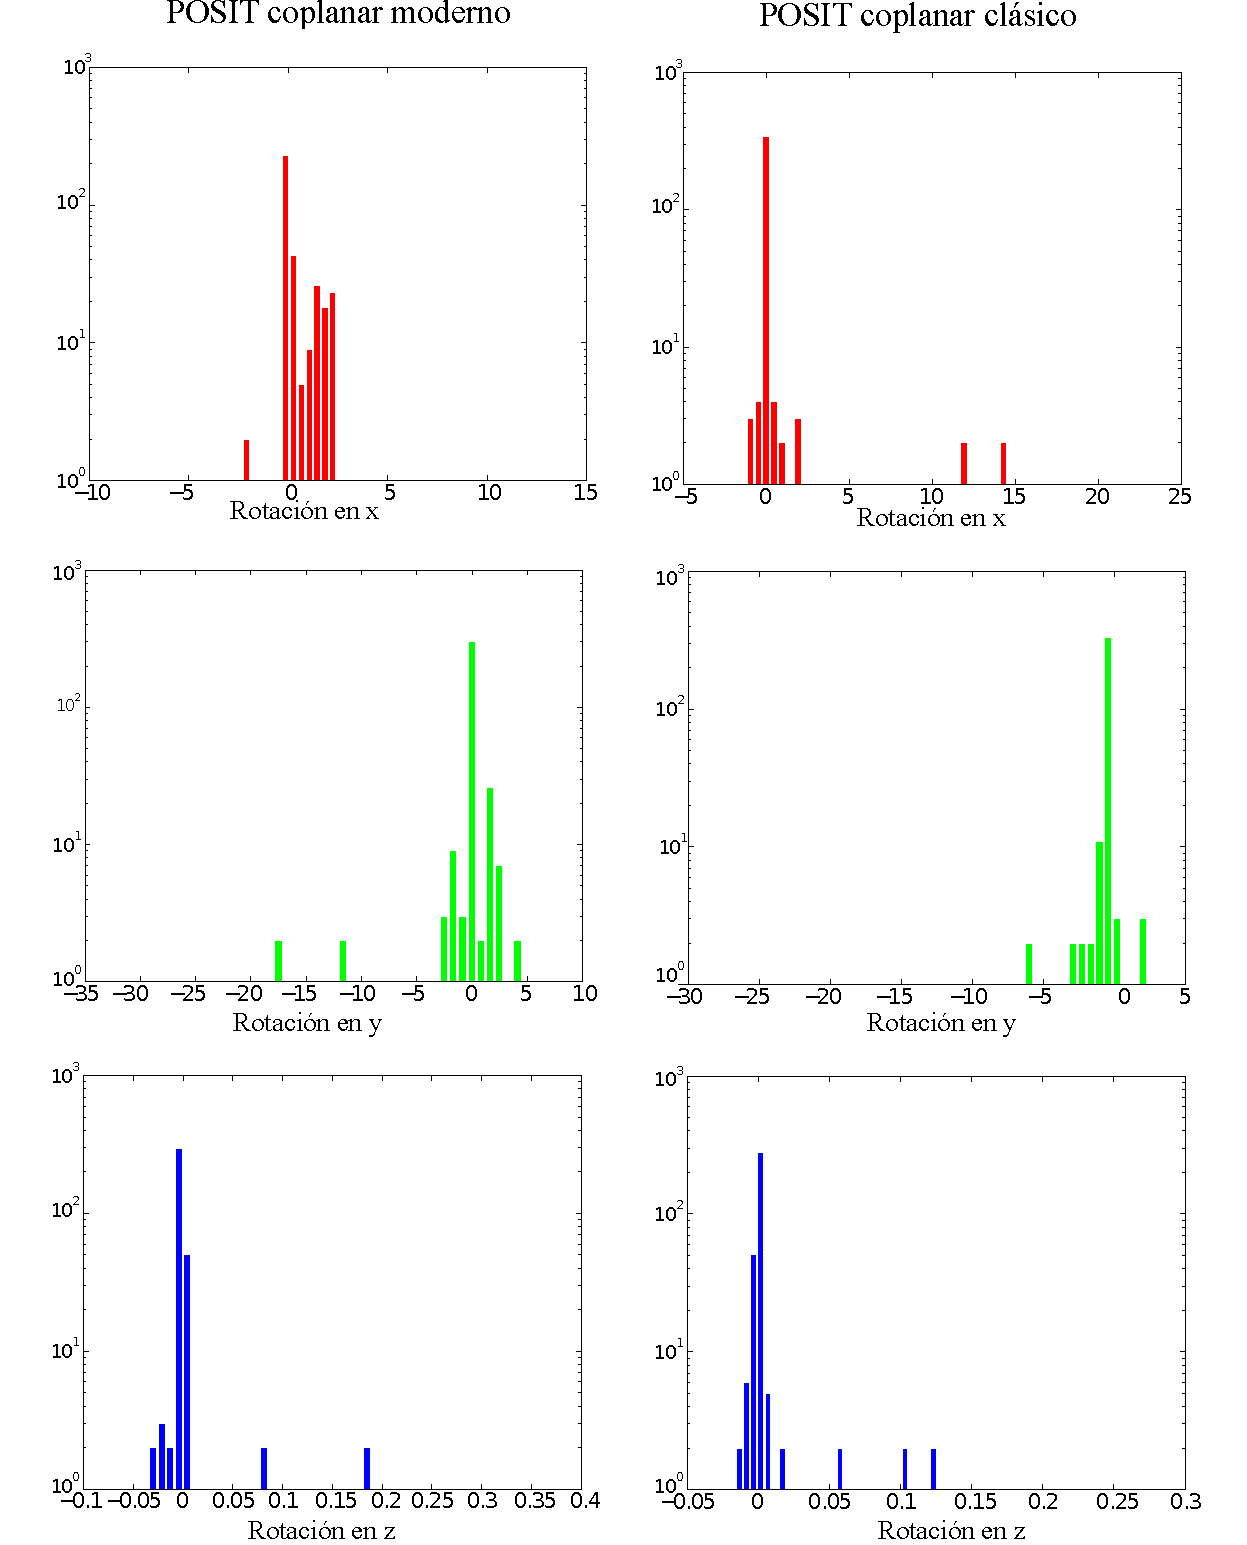
\includegraphics[scale=0.62]{figs_posit/histAngulosPosit2}
        \label{fig:posit_8}
         \caption{Histograma de los errores obtenidos en la orientaci�n. En la columna de la izquierda se muestran los resultados obtenidos para POSIT coplanar moderno seg�n \textit{x}, \textit{y}  y \textit{z}.  En la columna de la derecha se muestran los histogramas para POSIT coplanar cl�sico seg�n \textit{x}, \textit{y}  y \textit{z}. La escala de las gr�ficas es logar�tmica.}
\end{figure}


Se puede ver que los dos algoritmos se comportan de manera similar, en la mayor�a de los casos se obtiene un error de estimaci�n menor a $2^\circ$. Los casos en los que el error es mayor a  $2^\circ$ se corresponden con posiciones de la c�mara en las que el plano imagen es paralelo al plano del marcador. Este comportamiento se puede ver en la Figura \ref{fig:posit_9}. Si los �ngulos de rotaci�n en torno a $x$ o a $y$ est�n en un intervalo de $(-10^\circ,+10^\circ)$, la proyecci�n SOP del marcador var�a muy poco. Esto lleva a que el algoritmo termine eligiendo una pose que no es la correcta, o puede llevar a que el algoritmo no converja. 

\begin{figure}[ht]
\label{fig:posit_9}
        \centering
        \subfigure[]{
                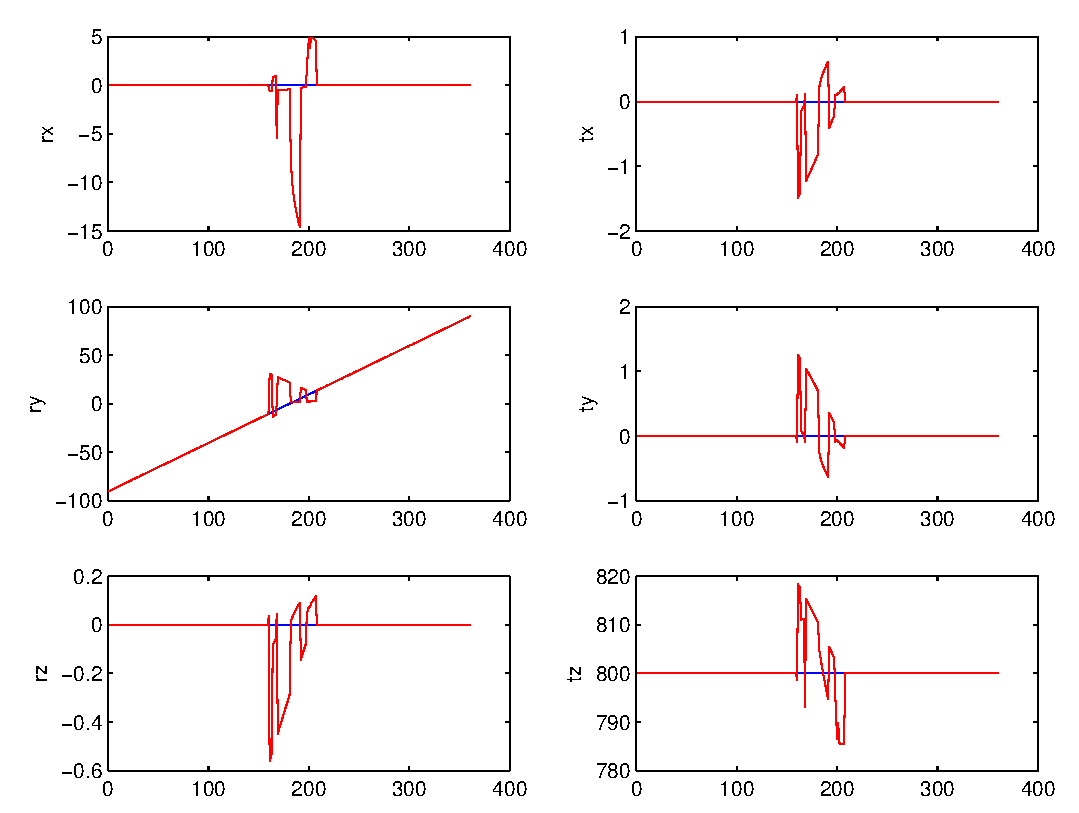
\includegraphics[scale=0.65]{figs_posit/barrido}
				\label{fig:posit_10}}
        \subfigure[]{
                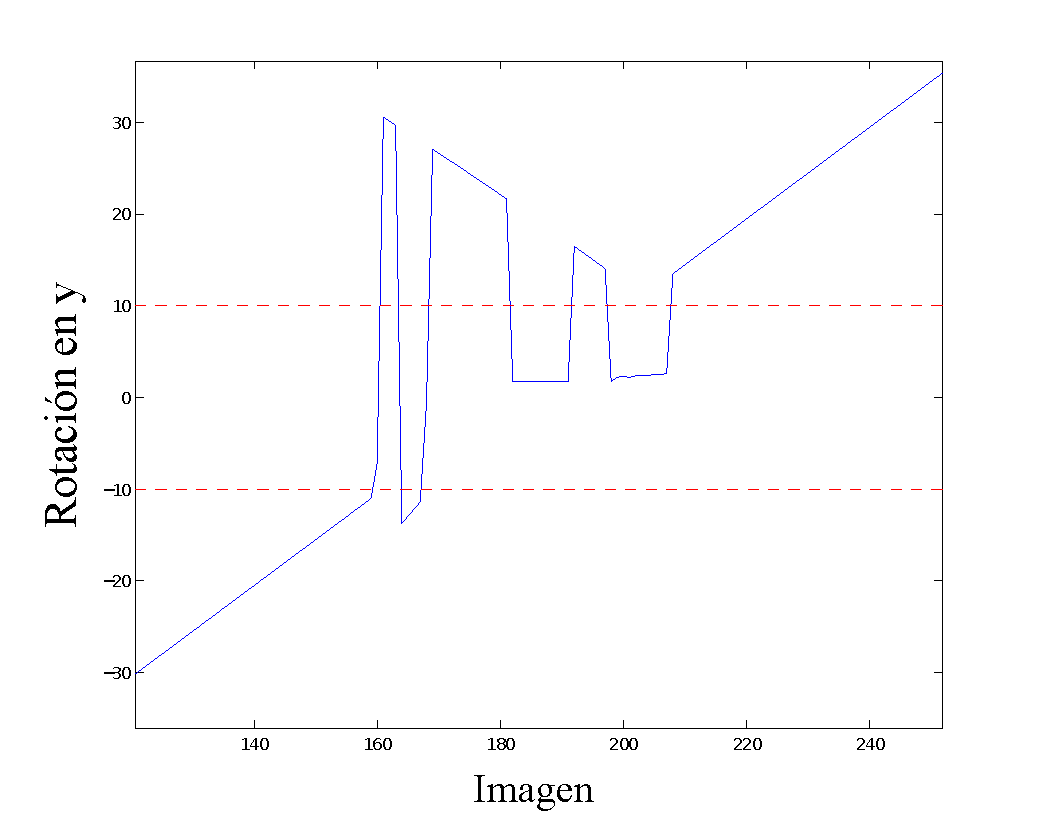
\includegraphics[scale=0.6]{figs_posit/zoom}
                \label{fig:posit_11}}
                
         \caption{En \subref{fig:posit_10} se puede ver un barrido de rotaciones respecto al eje $y$, solo hay error cuando el �ngulo de rotaci�n es peque\~no. En \subref{fig:posit_11} se puede ver mas de cerca el comportamiento en torno a cero, se grafican los limites aproximados para los cuales el algoritmo presenta problemas.}
\end{figure}
En la Figura \ref{fig:posit_11} se puede ver que el algoritmo no presenta problemas para posiciones de la c�mara que corresponden a im�genes del marcador muy deformadas por la perspectiva, �ngulos cercanos a $90^\circ$. Este l�mite est� dado por el filtro de correspondencias visto en \ref{ch:marcadores}.


\subsubsection{Error de posici�n}
En la Figura \ref{fig:posit_12} se muestran los errores de posici�n para los diferentes ejes, en general la estimaci�n de la posici�n es buena, en la mayor�a de los casos el error es menor al $1\% $ . Se vio que para las distancias al marcador a las que se trabaja el algoritmo no presenta problema, en este caso la limitante est� dada por el filtro de correspondencias presentado en \ref{ch:marcadores}. 

\begin{figure}[H]
\centering
        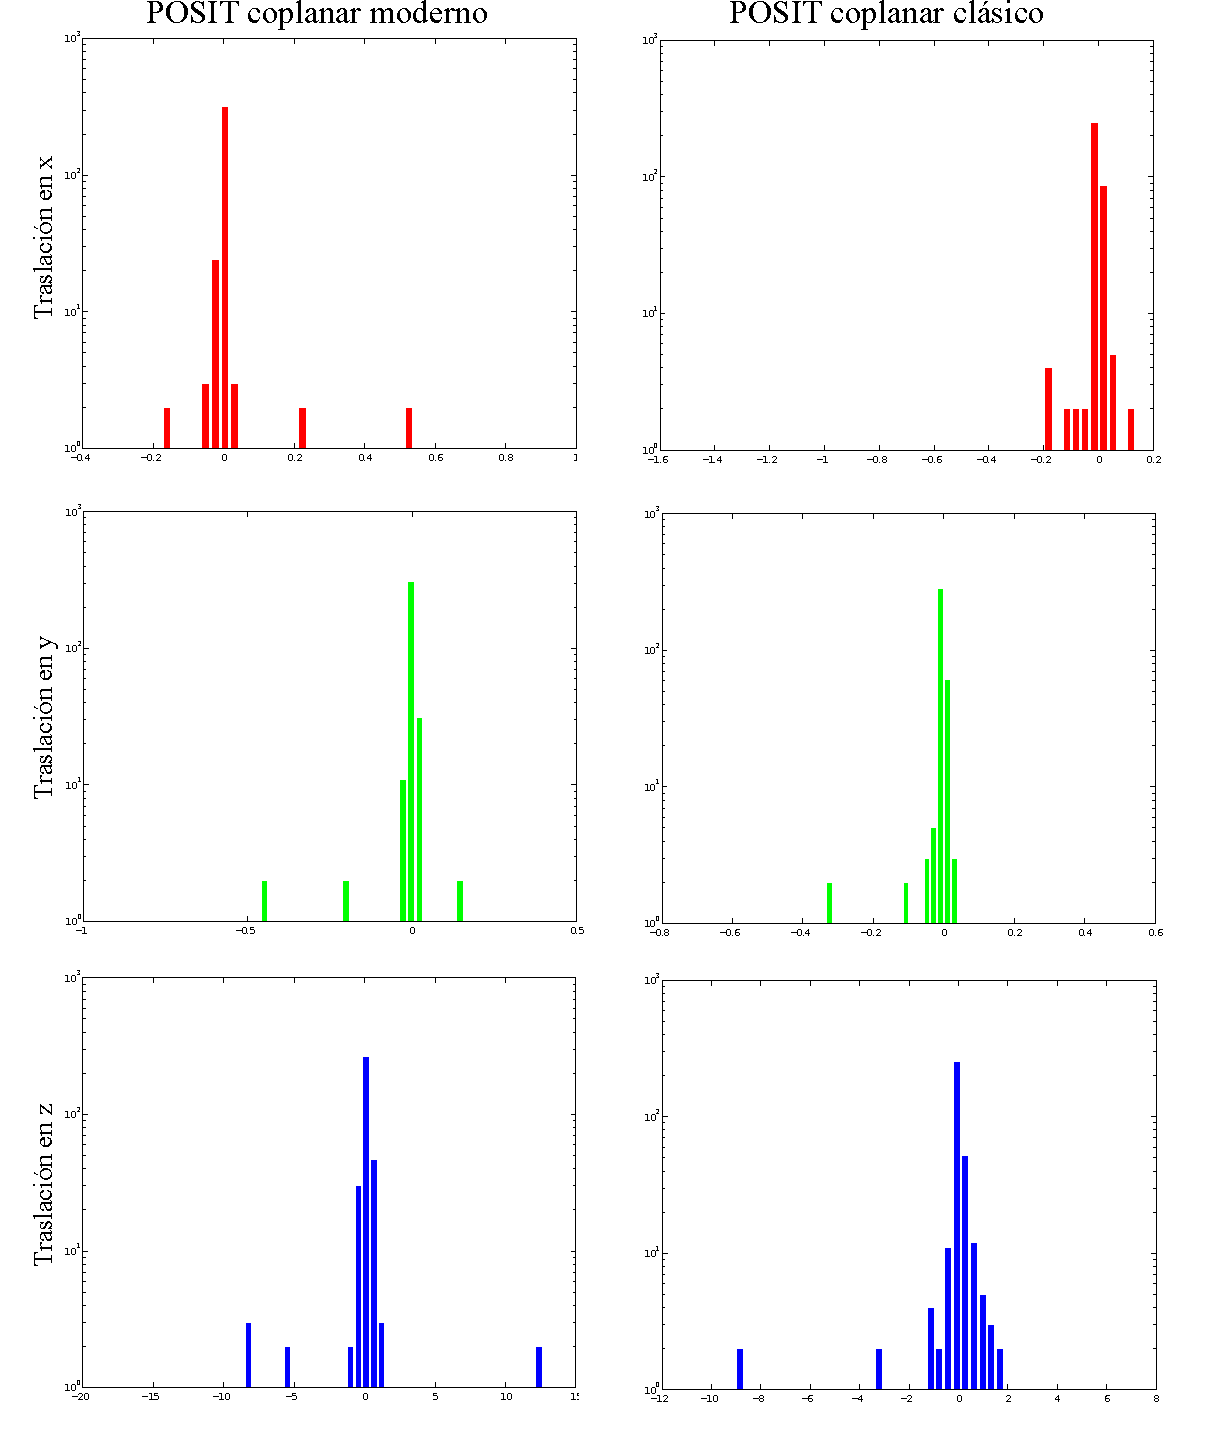
\includegraphics[scale=0.62]{figs_posit/histTrasPosit2}
        \label{fig:posit_12}
         \caption{Histograma de los errores obtenidos en traslaci�n En la columna de la izquierda se muestran los resultados obtenidos para POSIT coplanar moderno seg�n \textit{x}, \textit{y}  y \textit{z}.  En la columna de la derecha se muestran los histogramas para POSIT coplanar cl�sico seg�n \textit{x}, \textit{y}  y \textit{z}. La escala en el de las gr�ficas es logar�tmica.}
\end{figure}

\subsubsection{Comportamiento global}\label{sec: positComportamientoGlobal}
A continuaci�n se muestra el comportamiento de las dos variantes del algoritmo para una trayectoria representativa del movimiento que se realiza con el dispositivo. Se generaron 100 im�genes a partir de poses a las que se les sum� un ruido blanco para simular el comportamiento de una persona. La trayectoria se puede dividir en dos movimientos. 
\begin{figure}[H]
\label{fig:posit_13}
        \centering
        \subfigure[]{
                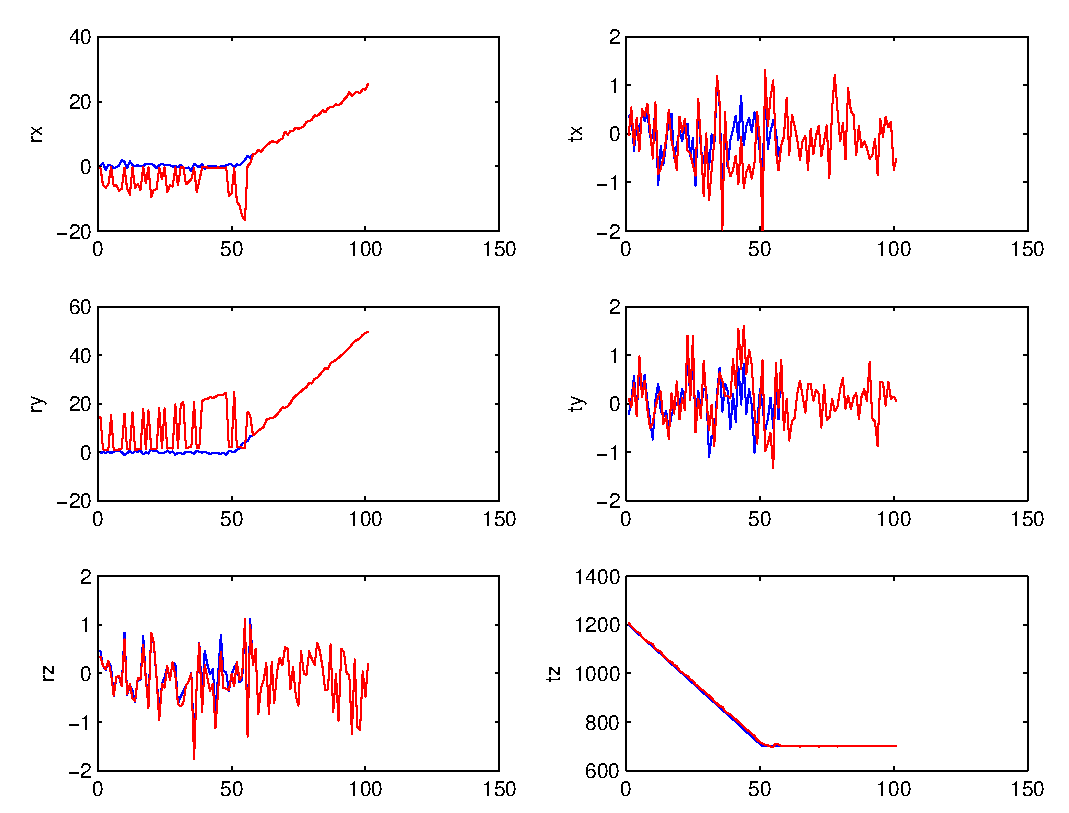
\includegraphics[scale=0.4]{figs_posit/recorridaCopl}
				\label{fig:posit_14}}
        \subfigure[]{
                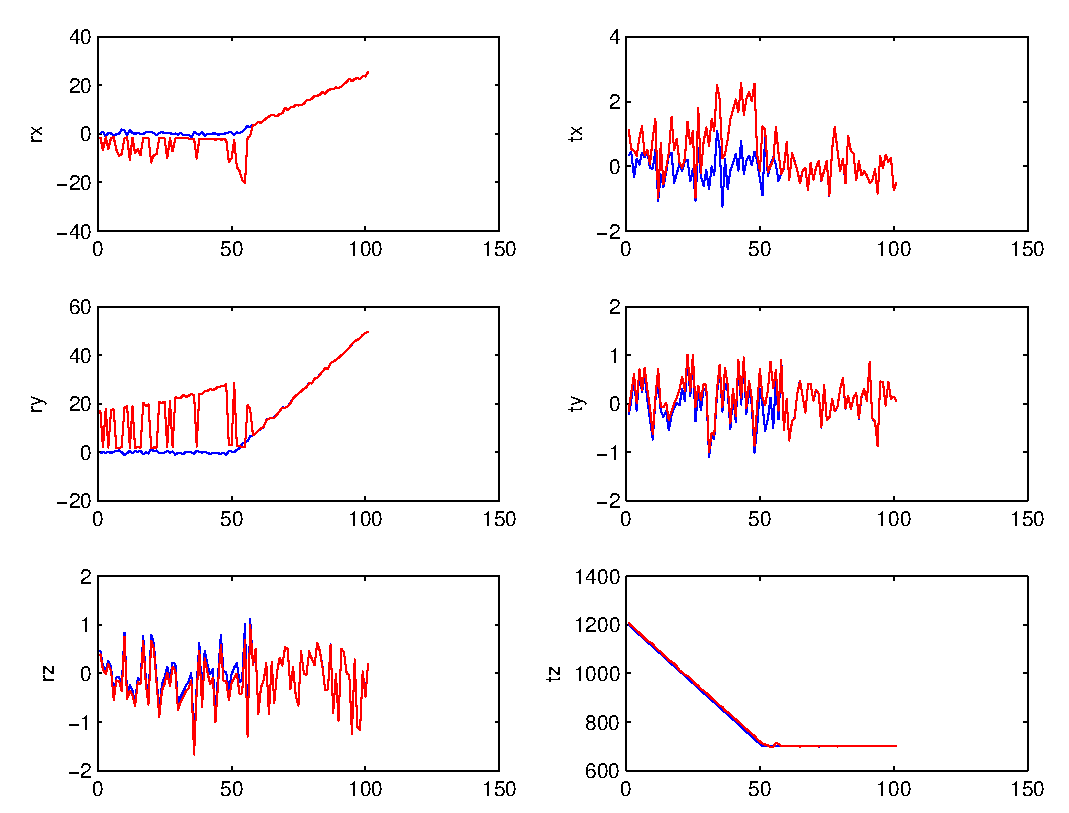
\includegraphics[scale=0.4]{figs_posit/recorridaComp}
                \label{fig:posit_15}}
                
         \caption{Trayectoria en la que se ve que el error es mayor cuando el marcador es visto de frente. Cuando se empieza a rotar el error de orientaci�n es chico. En la Figura \subref{fig:posit_14} se puede ver el comportamiento de POSIT coplanar moderno y en la Figura \subref{fig:posit_15} se puede ver el comportamiento para POSIT coplanar cl�sico.}
 \end{figure}

El primer movimiento simula la c�mara acerc�ndose al marcador. En este movimiento se puede ver c�mo ambos algoritmos fallan en la estimaci�n de la pose. La versi�n moderna comete menos error. El segundo movimiento se tiene a la c�mara en una posici�n fija y va cambiando su orientaci�n, se puede apreciar que para este caso el error cometido en orientaci�n es muy peque\~no. 

Si bien el comportamiento de los dos algoritmos result� similar, la versi�n de POSIT coplanar moderno dio resultados levemente mejores que la versi�n cl�sica. Adem�s en la pr�ctica se comport� mejor por lo que esta versi�n es la que se utiliza en la aplicaci�n final. 

\section{Error de reproyecci�n}

Se utilizaron im�genes de prueba obtenidas con el \textit{iPad 2} e im�genes sint�ticas. Para ambos grupos de im�genes se midi� el error de proyecci�n obtenido entre los puntos del modelo y los puntos detectados. 

Para el caso de las im�genes de prueba del \textit{iPad} se eligieron 9 posiciones y en cada posici�n se sacaron 50 fotos. Con estas 450 fotos se obtuvo la estad�stica del funcionamiento de los algoritmos. En la Figura \ref{fig:posit_16} se puede ver una de las im�genes utilizadas para cada posici�n. Tambi�n se utilizaron im�genes sint�ticas en posiciones similares a las de las im�genes de prueba que se pueden ver en la Figura \ref{fig:posit_20}, se utilizaron 9 casos con 50 fotos por caso. Se parti� de una posici�n base y se vari� la posici�n muy poco, intentando simular el movimiento que se  tuvo al sacar las fotos con el \textit{iPad}. En total se probaron 900 im�genes. 


 


 
A las im�genes se les aplica todo el proceso, se realiza la detecci�n y filtrado de segmentos, se calculan las correspondencias y luego se estima la pose. Para cada imagen se calcula el error de proyecci�n de cada punto, luego se promedian obteniendo una sola medida de error por imagen, esta medida es a su vez promediada con los errores obtenidos de la im�genes para un mismo caso. Esto sirve para evaluar el comportamiento de los algoritmos ya que los puntos a la entrada son los mismos para las dos variantes. En las tablas hay valores que no pudieron ser calculados debido a que el filtro de segmentos no pudo detectar todos los segmentos. Estos comportamientos fueron discutidos en \ref{ch:detection}. 

\begin{figure}[H]
\centering
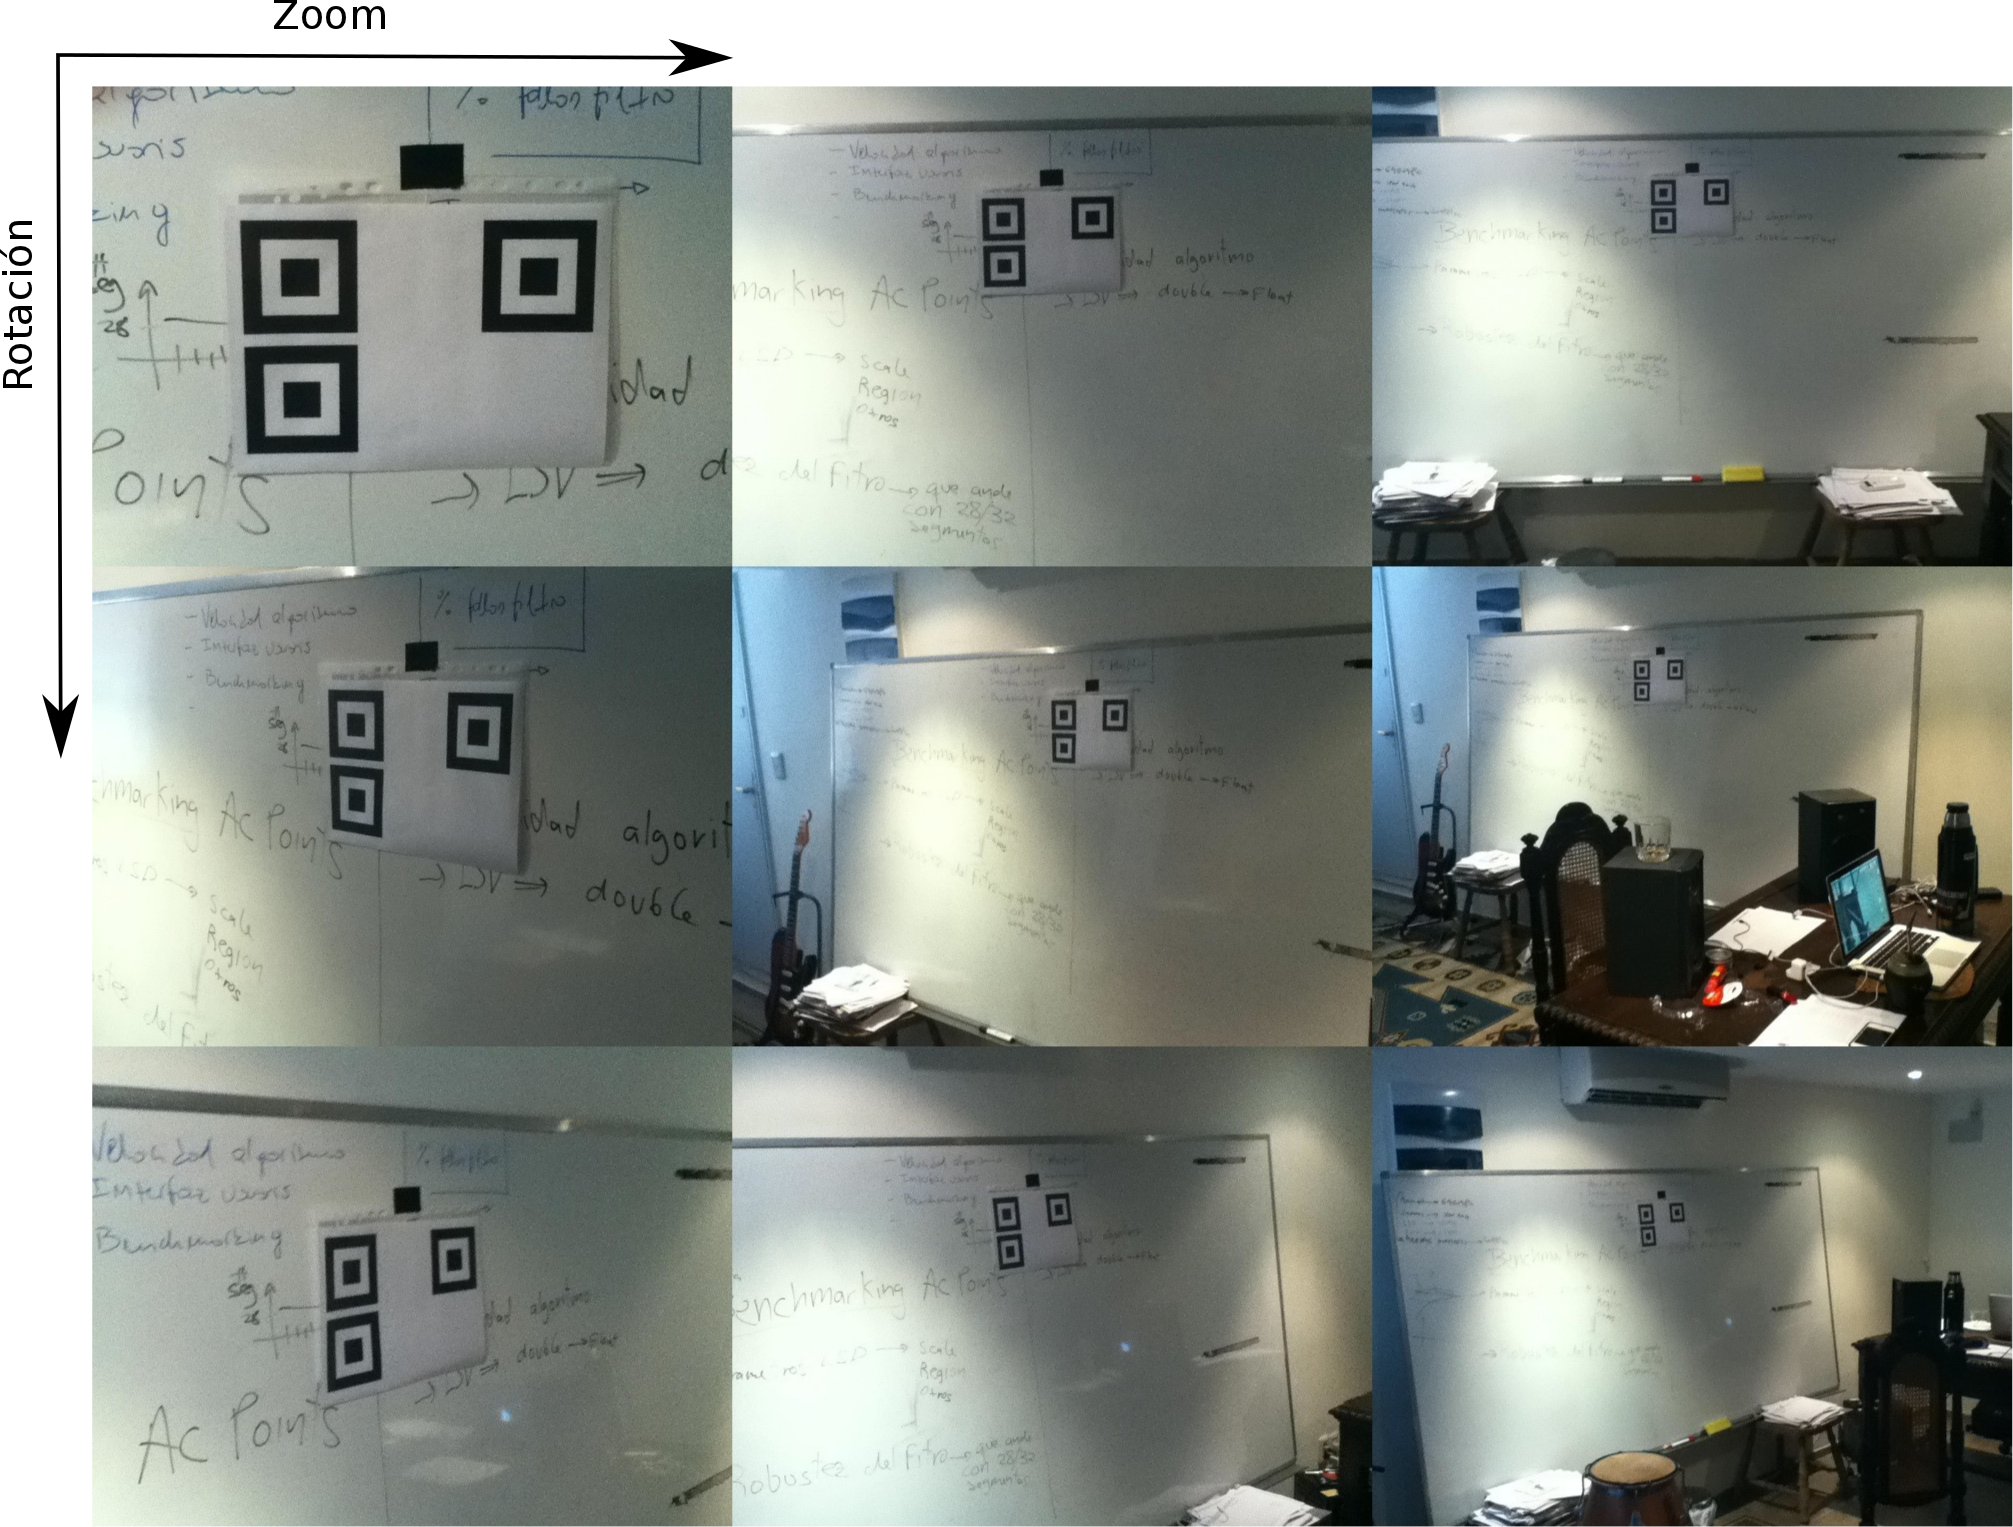
\includegraphics[scale=0.2]{figs_posit/posit_8b}
\label{fig:posit_16}
\caption{Posiciones que se utilizaron para las im�genes de prueba.}
\end{figure}

\begin{figure}[H]
\label{fig:posit_17}
        \centering
        \subfigure[]{
                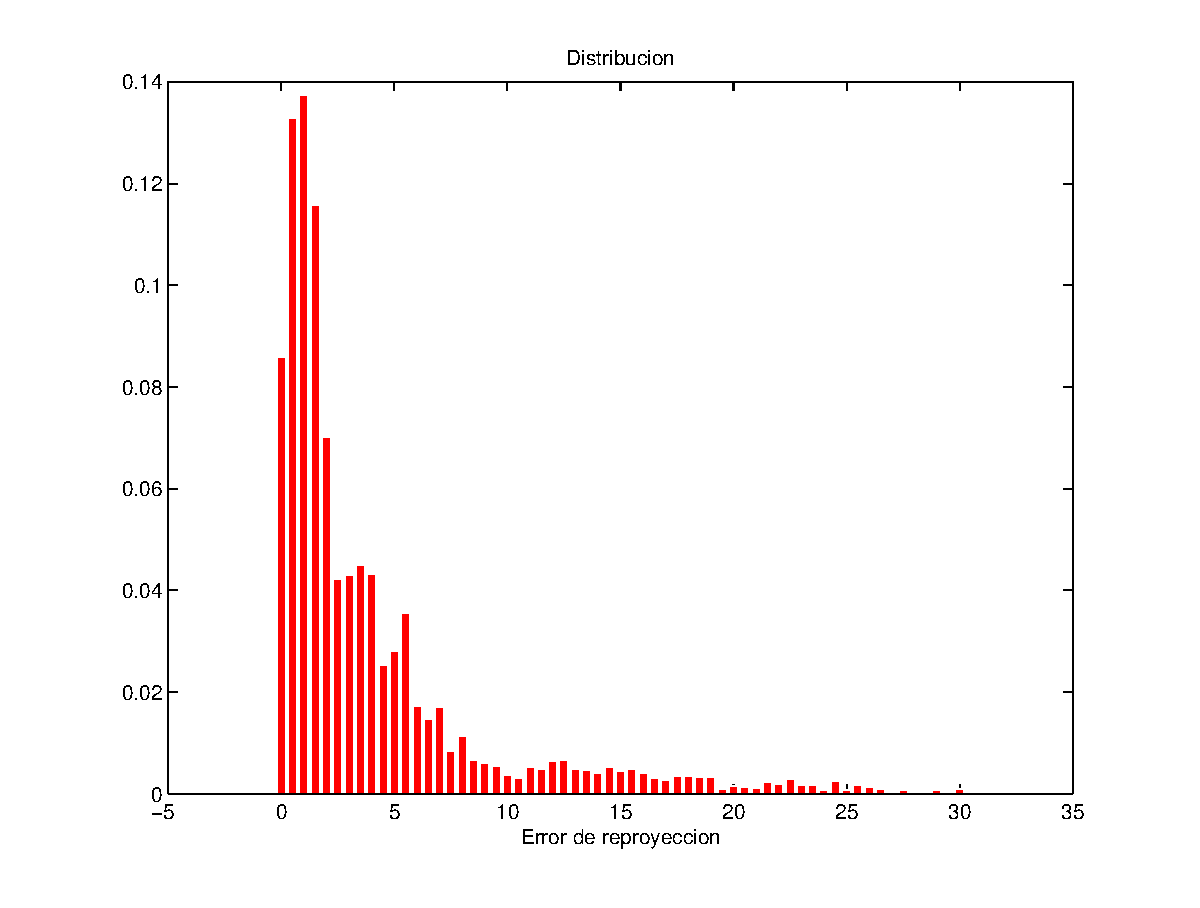
\includegraphics[scale=0.4]{figs_posit/histDistEuclCopl}
				\label{fig:posit_18}}
        \subfigure[]{
                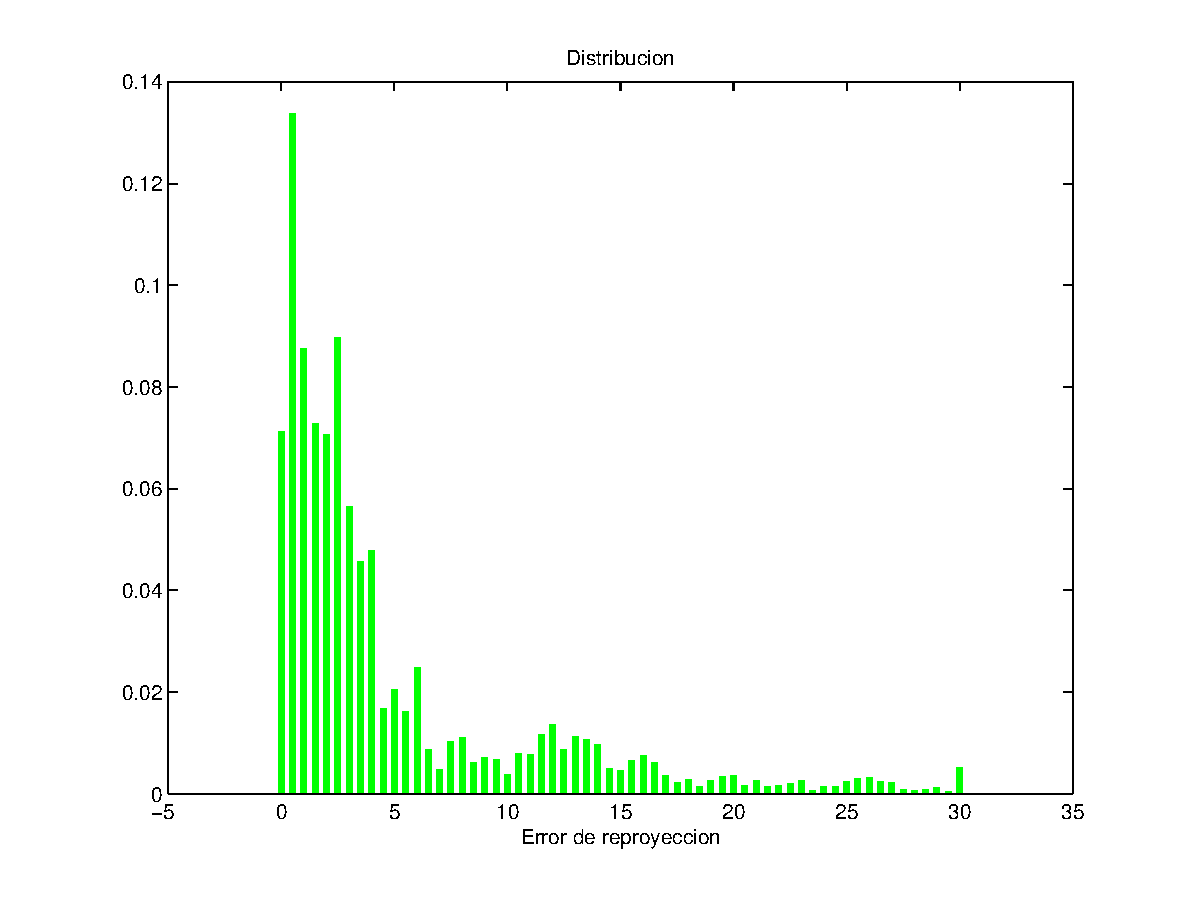
\includegraphics[scale=0.4]{figs_posit/histDistEuclComp}
                \label{fig:posit_19}}
                
         \caption{Histograma normalizado de los errores de reproyecci�n para POSIT para las im�genes de prueba. \subref{fig:posit_18}, POSIT moderno. \subref{fig:posit_19}, POSIT cl�sico}
 \end{figure}

\begin{table}[H]
\centering
\begin{tabular}{|l||r|r|}
\hline
 & \multicolumn{1}{l|}{\textbf{Modern POSIT}} & \multicolumn{1}{l|}{\textbf{Classic POSIT}} \\ \hline \hline
\textbf{Media} & 3.9684 &  5.1368  \\ \hline
\textbf{Desviaci�n est�ndar} &   5.1212 &     6.8950 \\ \hline
\end{tabular}
\caption{Error de proyecci�n de im�genes de pruebas. El error est� expresado en p�xeles}
\label{posit_tabla1}
\end{table} 

\begin{figure}[ht]
\centering
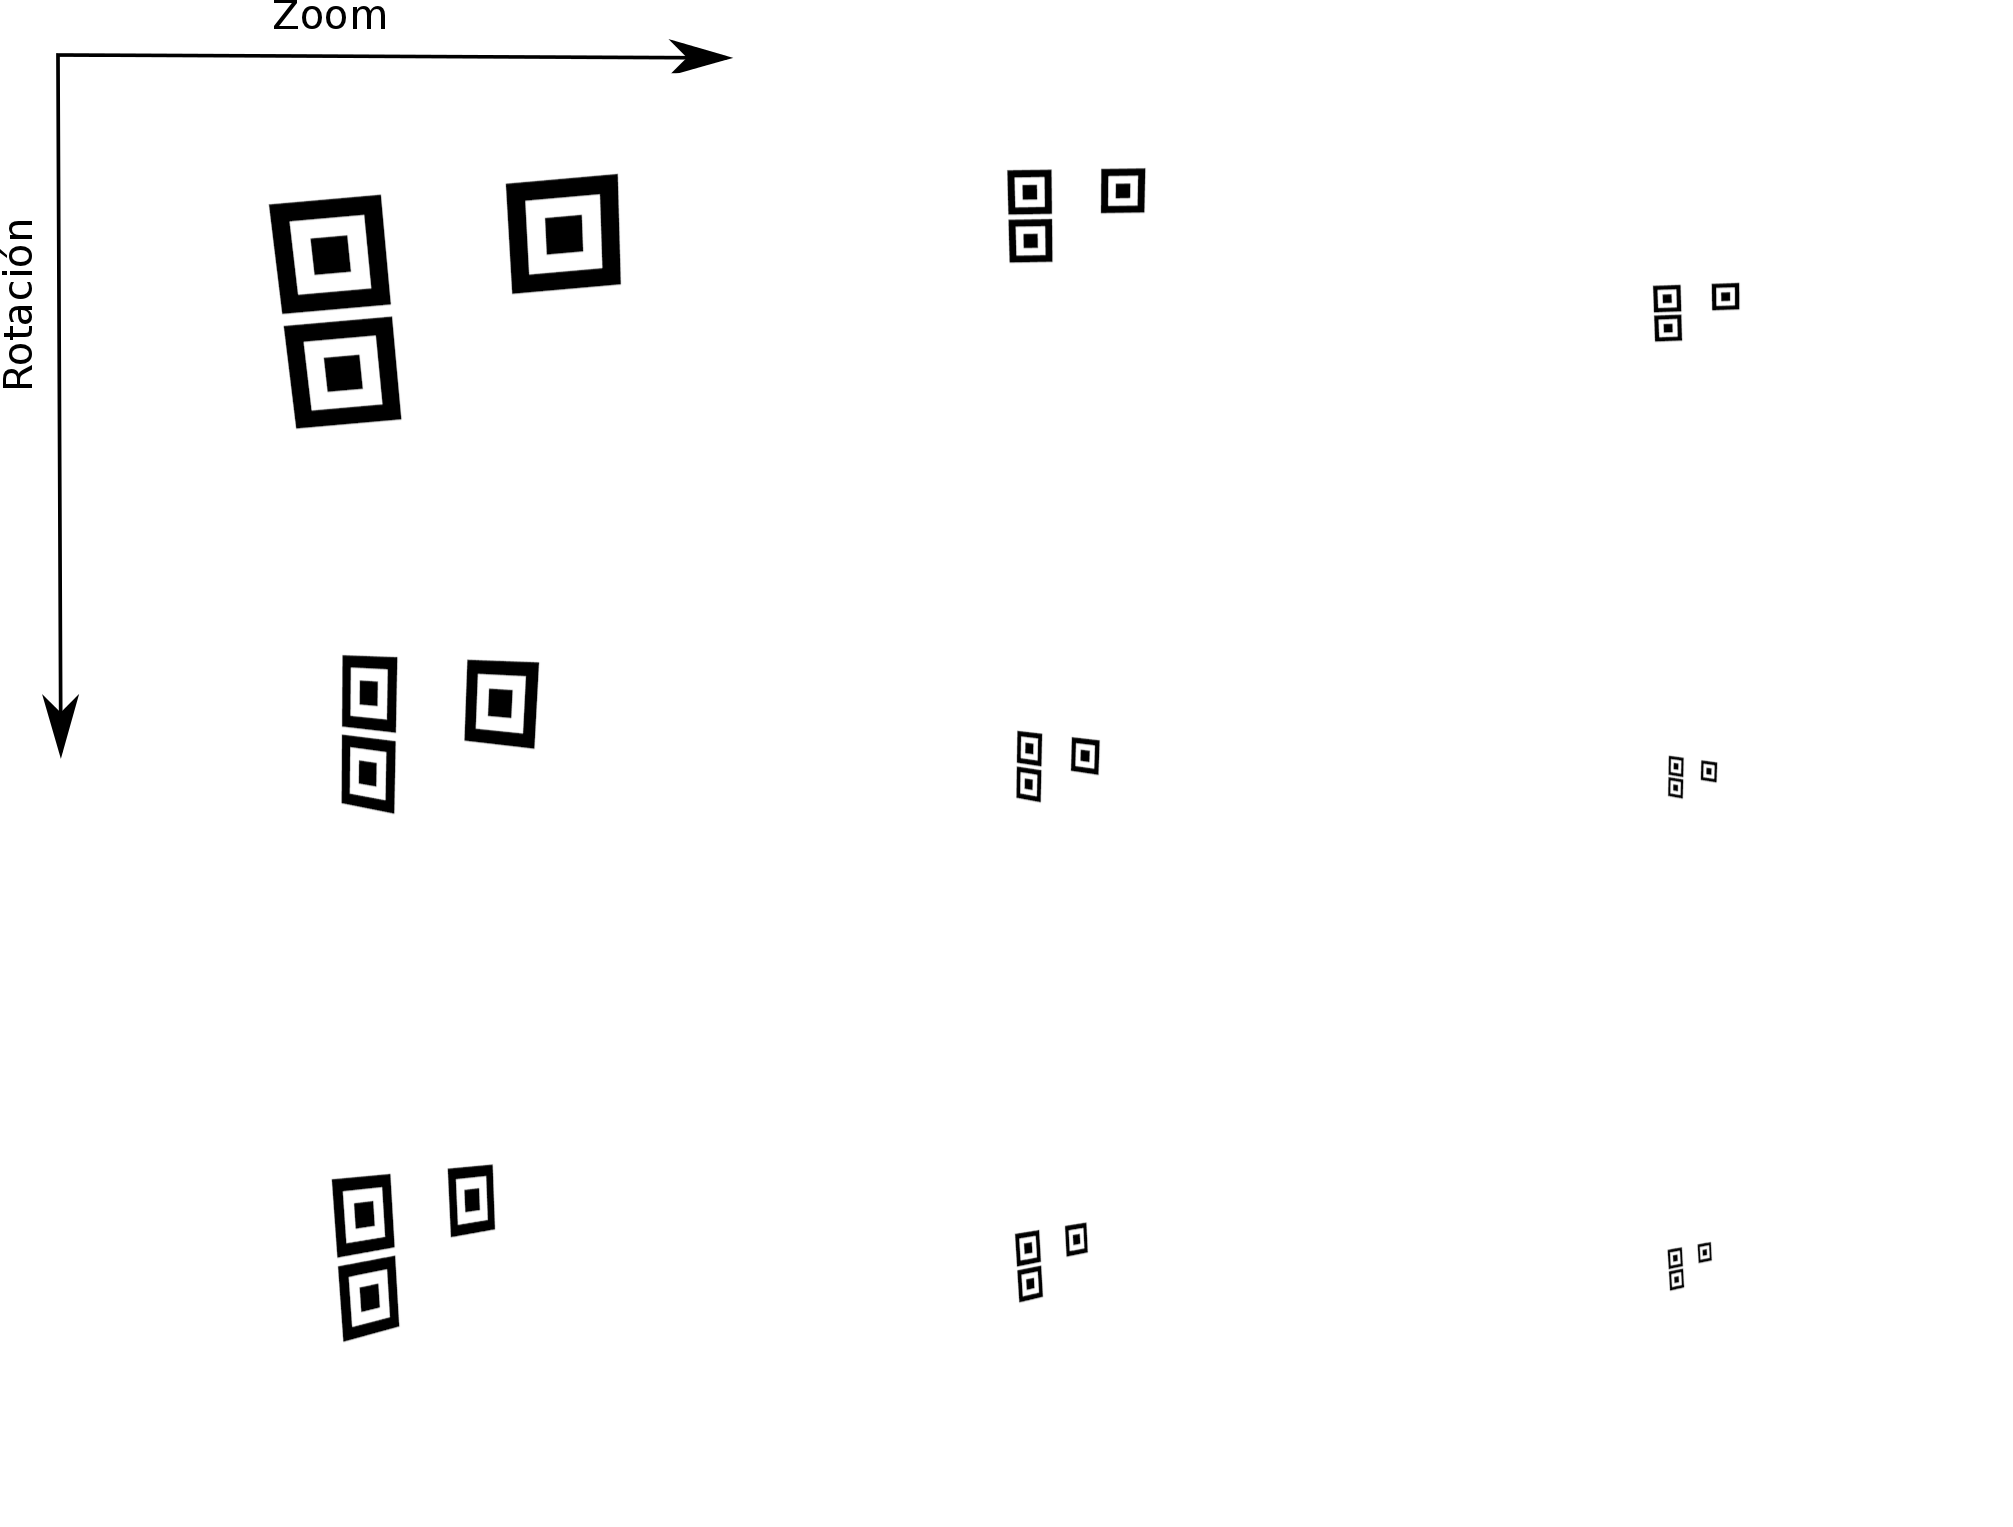
\includegraphics[scale=0.2]{figs_posit/posit_9b}
\label{fig:posit_20}
\caption{Posiciones que se utilizaron para las im�genes sint�ticas}
\end{figure}

\begin{figure}[H]
\label{fig:posit_21}
        \centering
        \subfigure[]{
                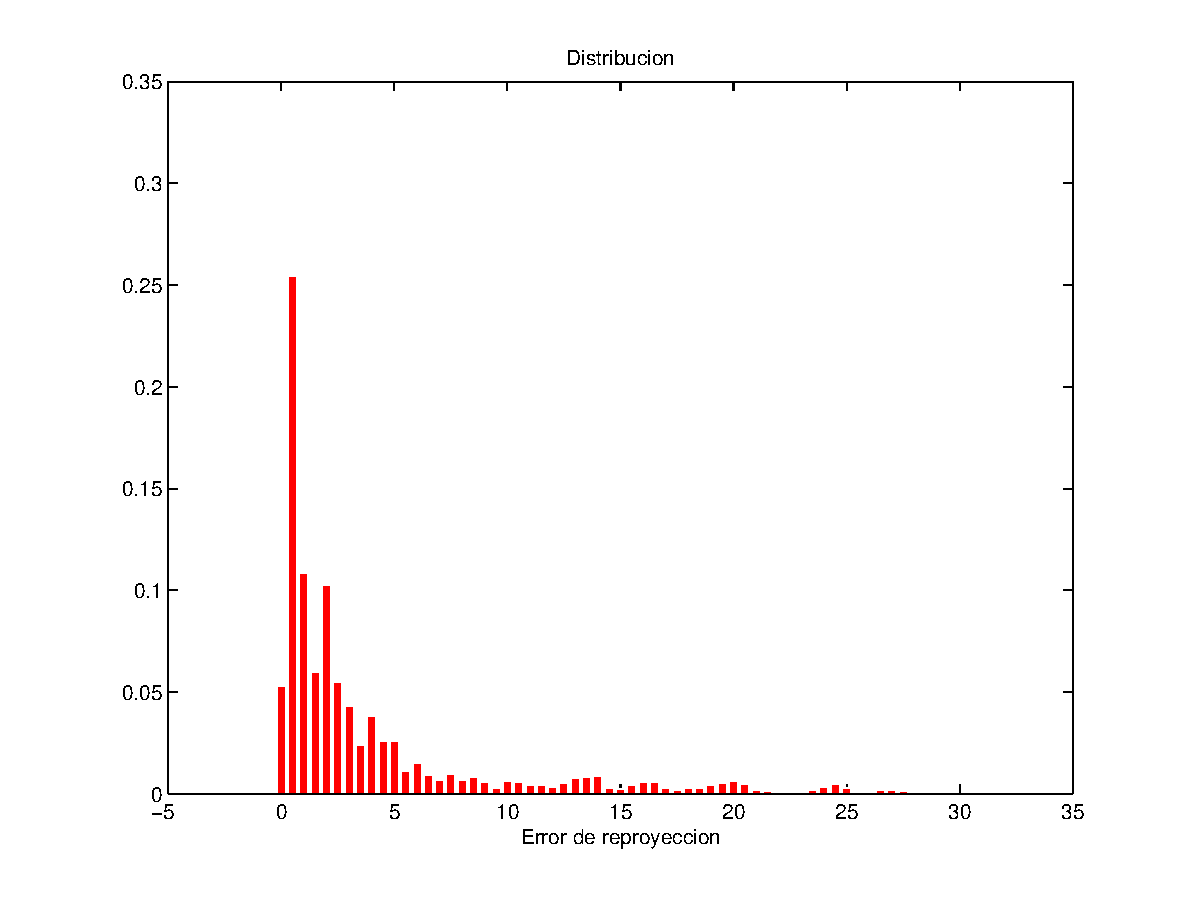
\includegraphics[scale=0.4]{figs_posit/histDistEuclCoplSint}
				\label{fig:posit_22}}
        \subfigure[]{
                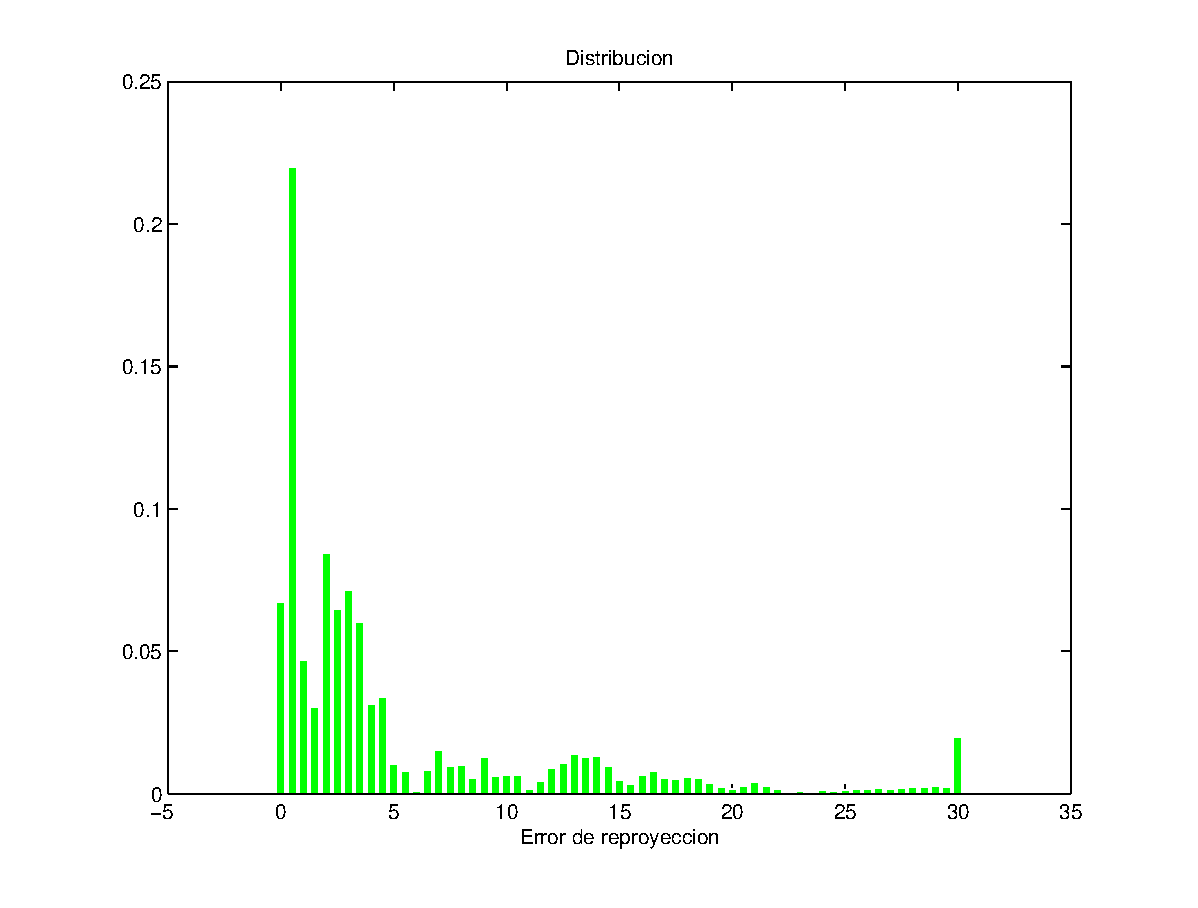
\includegraphics[scale=0.4]{figs_posit/histDistEuclCompSint}
                \label{fig:posit_23}}
                
         \caption{Histograma normalizado de los errores de reproyecci�n para POSIT para las im�genes sint�ticas. \subref{fig:posit_22}, POSIT moderno. \subref{fig:posit_23}, POSIT cl�sico}
 \end{figure}

\begin{table}[ht]
\centering
\begin{tabular}{|l||r|r|}
\hline
 & \multicolumn{1}{l|}{\textbf{Modern POSIT}} & \multicolumn{1}{l|}{\textbf{Classic POSIT}} \\ \hline \hline
\textbf{Media} & 4.033 &  5.4942  \\ \hline
\textbf{Desviaci�n est�ndar} &   5.6196 &    7.2591 \\ \hline
\end{tabular}
\caption{Error de proyecci�n de im�genes sint�ticas. El error est� expresado en p�xeles}
\label{posit_tabla2}
\end{table} 


%\begin{table}[htbp]
%\centering
%\begin{tabular}{|l||r|r|r|r|}
%\hline
% & \multicolumn{1}{l|}{\textbf{Modern POSIT}} & \multicolumn{1}{l|}{\textbf{Varianza}} & \multicolumn{1}{l|}{\textbf{Classic POSIT}} & \multicolumn{1}{l|}{\textbf{Varianza}} \\ \hline \hline
%\textbf{Caso1} &   4.2712 &     0.3192 &     5.7352 &     0.4525 \\ \hline
%\textbf{Caso2} &     1.0831 &     0.0375 &     1.0889 &     0.0358 \\ \hline
%\textbf{Caso3} &        - &        - &        - &        - \\ \hline
%\textbf{Caso4} &     0.7975 &     0.0169 &     0.9778 &     0.0185 \\ \hline
%\textbf{Caso5} &        - &        - &        - &        - \\ \hline
%\textbf{Caso6} &        - &        - &        - &        - \\ \hline
%\textbf{Caso7} &     0.3796 &     0.0121 &     0.4761 &     0.0077 \\ \hline
%\textbf{Caso8} &        - &        - &        - &        - \\ \hline
%\textbf{Caso9} &        - &        - &        - &        - \\ \hline
%\end{tabular}
%\caption{Error de proyecci�n en im�genes sint�ticas}
%\label{posit_tabla2}
%\end{table}

%Para otro grupo de im�genes sint�ticas se compar� la pose original con la pose obtenida luego de aplicar el procesamiento, se relev� el desempe\~no de los algoritmos para rotaciones seg�n los tres ejes. En general se vio que la implementaci�n de  POSIT moderno dio mejores resultados. 
%En la Figura \ref{fig:posit_16} se pueden algunos de los resultados obtenidos de la comparaci�n de desempe\~no de los dos algoritmos implementados. En la columna de la izquierda se muestran los resultados de POSIT moderno y en la de la derecha los resultados para POSIT cl�sico. 
%\begin{figure}\label{fig:posit_16}
%        \centering
%        \subfigure[]{
%                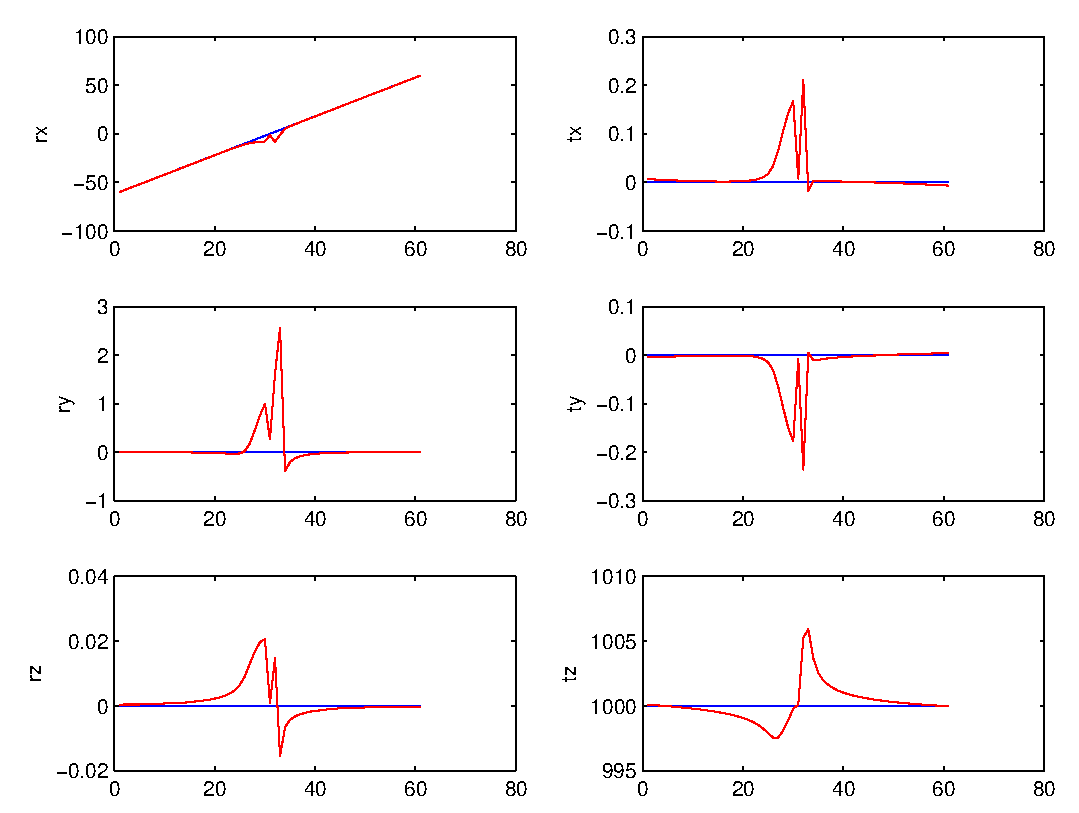
\includegraphics[scale=0.44]{figs_posit/poses_coplanar_scale3}
%				\label{fig:posit_10}}
%        \subfigure[]{
%                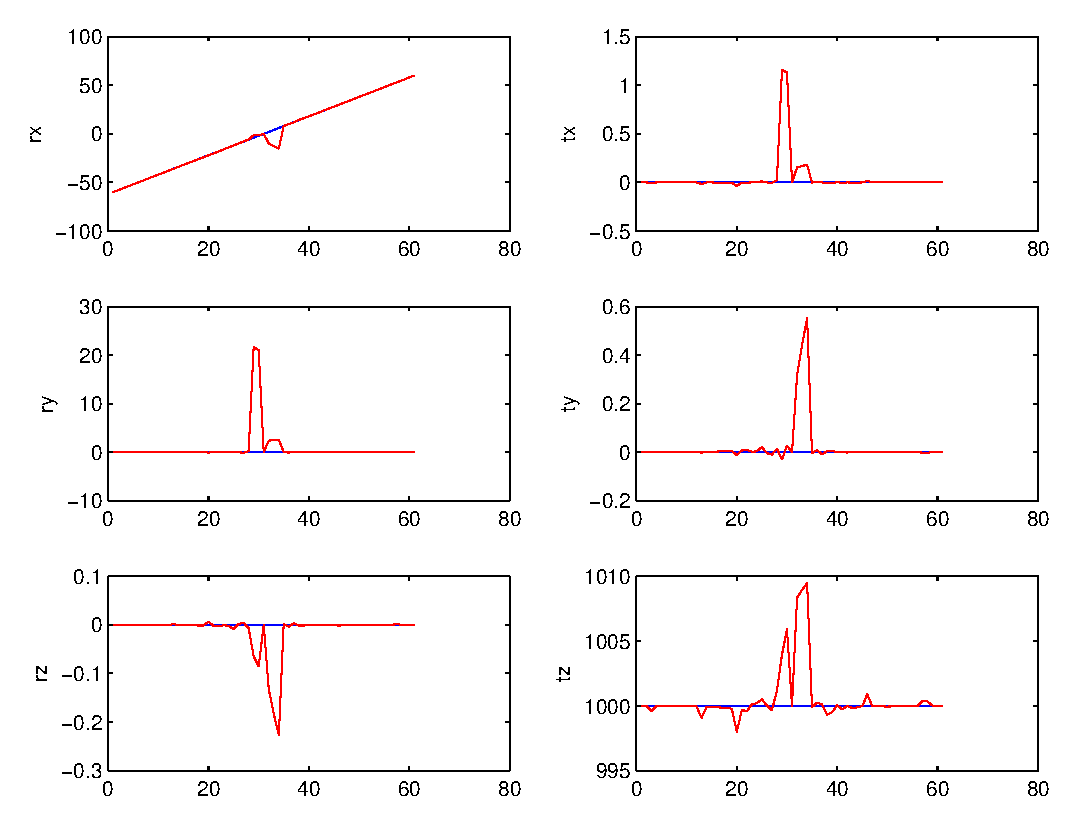
\includegraphics[scale=0.44]{figs_posit/poses_composit_scale3}
%                \label{fig:posit_11}}
%        
%       \subfigure[]{
%                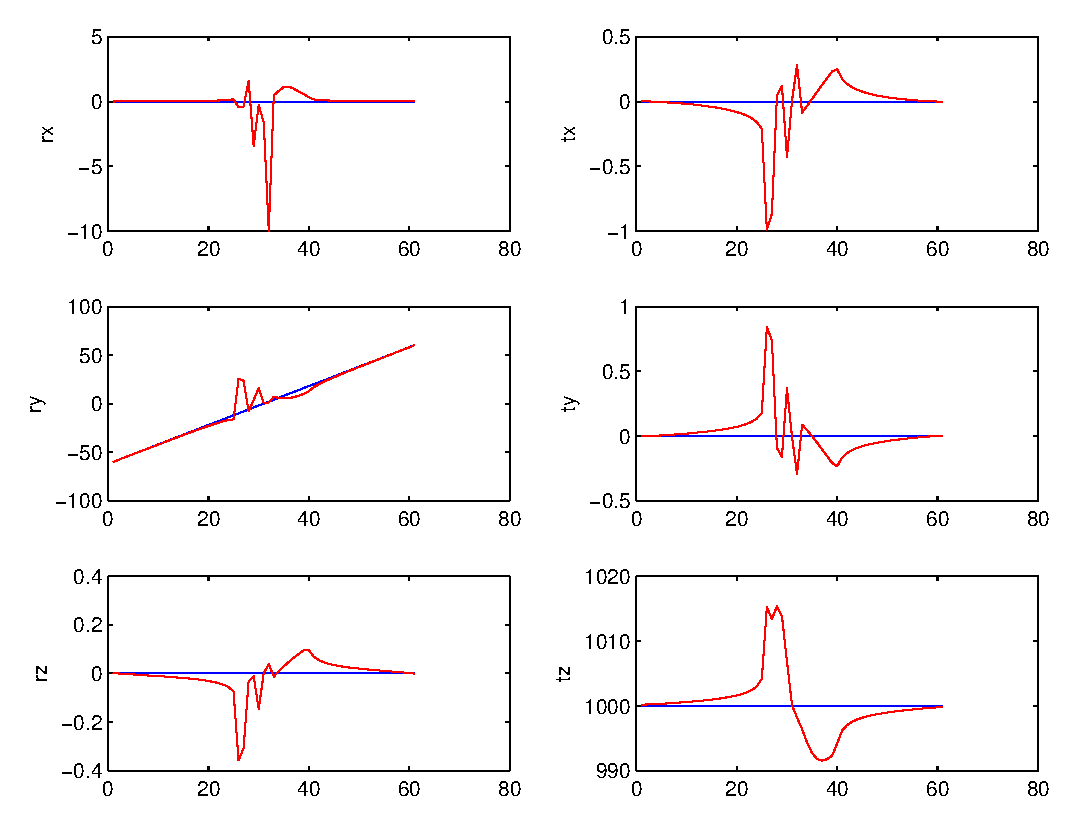
\includegraphics[scale=0.44]{figs_posit/poses_coplanar_scale4}
%				\label{fig:posit_12}}
%        \subfigure[]{
%                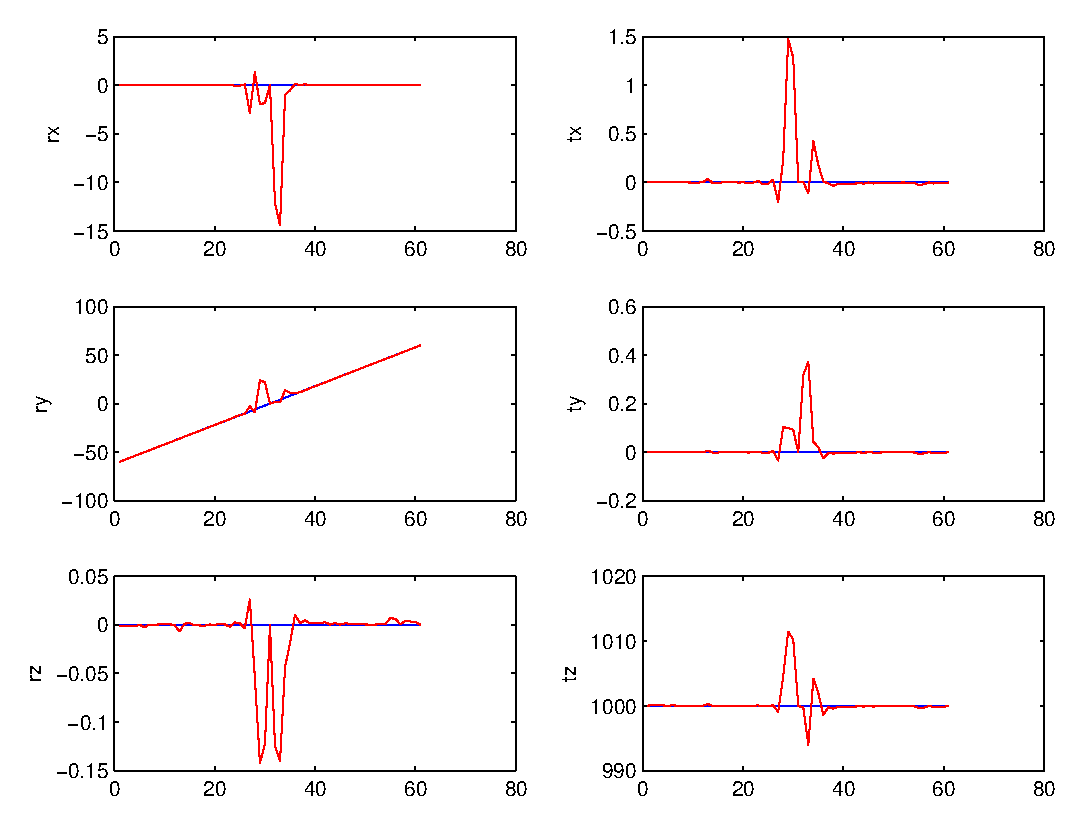
\includegraphics[scale=0.44]{figs_posit/poses_composit_scale4}
%                \label{fig:posit_13}}
%        
%        \subfigure[]{
%                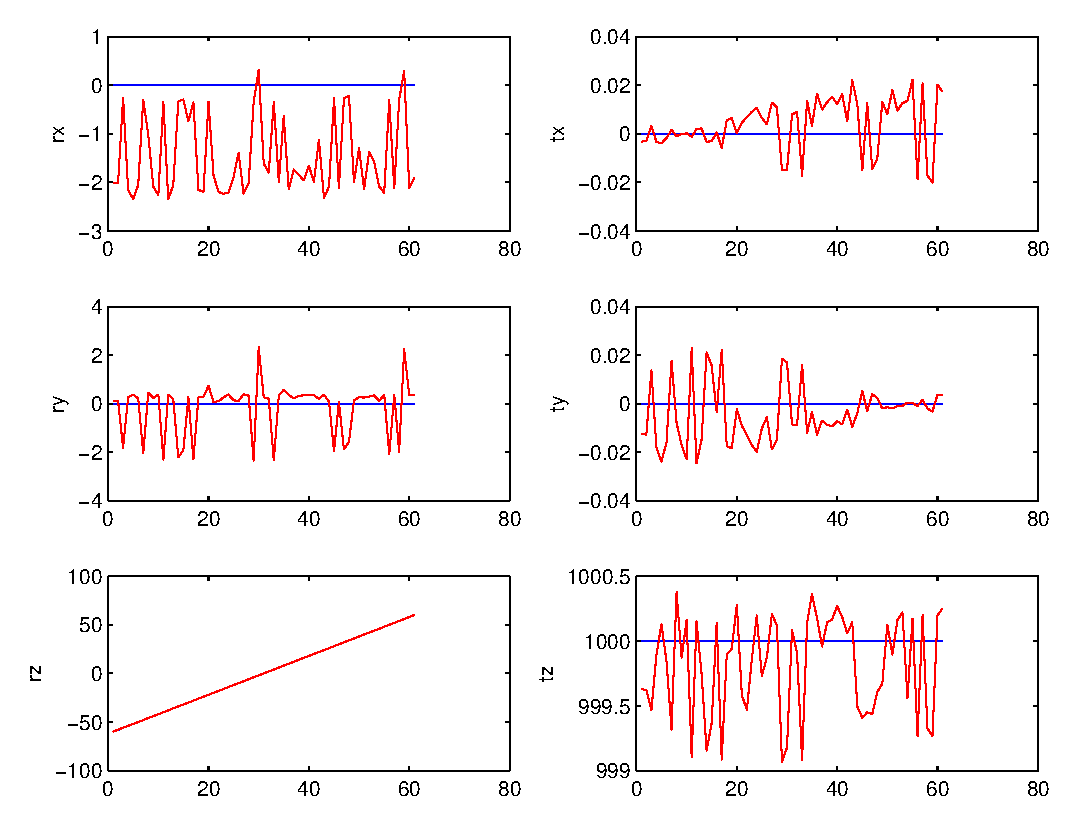
\includegraphics[scale=0.44]{figs_posit/poses_coplanar_scale5}
%				\label{fig:posit_14}}
%        \subfigure[]{
%                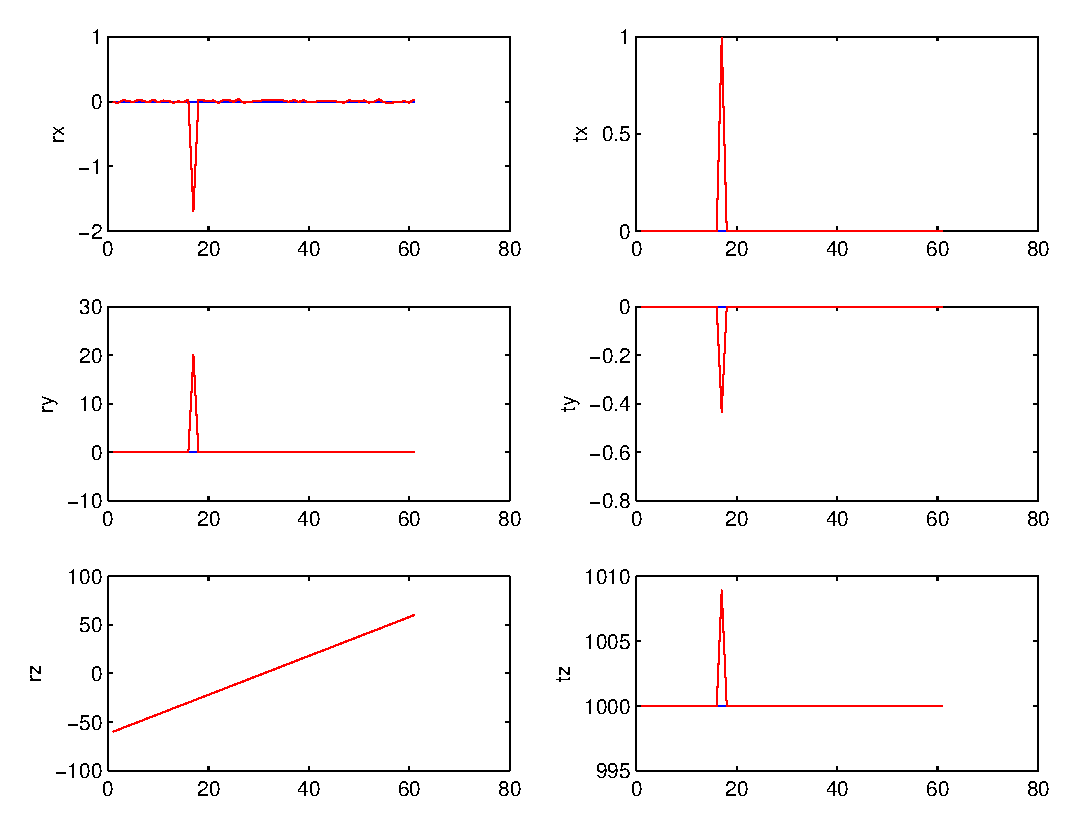
\includegraphics[scale=0.44]{figs_posit/poses_composit_scale5}
%                \label{fig:posit_15}}
%         \caption{Rotaci�n seg�n eje \textit{x} para Modern POSIT \subref{fig:posit_10} y para Classic POSIT \subref{fig:posit_11}, rotaci�n seg�n eje \textit{y} para Modern POSIT \subref{fig:posit_12} y para Classic POSIT \subref{fig:posit_13} y rotaci�n seg�n eje \textit{z} para Modern POSIT \subref{fig:posit_14} y para Classic POSIT \subref{fig:posit_15}}
%\end{figure}




En general se puede ver que el error de proyecci�n y la varianza son un poco menores para el caso de POSIT coplanar moderno.  Esto justifica la elecci�n del POSIT coplanar moderno. 

\section{Resumen}
En este cap�tulo se present� la teor�a detr�s del algoritmo POSIT. Se explicaron las diferentes versiones que se utilizaron, se vio que para marcadores coplanares hay ambig�edad en la estimaci�n de la pose lo que genera errores. Se present� una variante del POSIT coplanar moderno que minimiza una funci�n de costo para estimar la pose, a diferencia de la versi�n cl�sica que resuelve la estimaci�n utilizando m�nimos cuadrados. Tambi�n se explic� el algoritmo SoftPOSIT que estima las pose para conjuntos de puntos para los cuales no se saben las correspondencias. Este algoritmo requiere de una pose inicial para realizar la b�squeda. 

Se realiz� un estudio detallado del desempe\~no de los las dos versiones de POSIT coplanar y se compararon los resultados obtenidos, se vio que las dos versiones funcionan de manera similar.




% Ejemplo de como hacer una cita:
\cite{Daniel03simultaneouspose}.



\bibliographystyle{unsrt}   
\bibliography{encuadro}  
\end{document}